% Options for packages loaded elsewhere
\PassOptionsToPackage{unicode}{hyperref}
\PassOptionsToPackage{hyphens}{url}
%
\documentclass[
]{book}
\usepackage{lmodern}
\usepackage{amssymb,amsmath}
\usepackage{ifxetex,ifluatex}
\ifnum 0\ifxetex 1\fi\ifluatex 1\fi=0 % if pdftex
  \usepackage[T1]{fontenc}
  \usepackage[utf8]{inputenc}
  \usepackage{textcomp} % provide euro and other symbols
\else % if luatex or xetex
  \usepackage{unicode-math}
  \defaultfontfeatures{Scale=MatchLowercase}
  \defaultfontfeatures[\rmfamily]{Ligatures=TeX,Scale=1}
\fi
% Use upquote if available, for straight quotes in verbatim environments
\IfFileExists{upquote.sty}{\usepackage{upquote}}{}
\IfFileExists{microtype.sty}{% use microtype if available
  \usepackage[]{microtype}
  \UseMicrotypeSet[protrusion]{basicmath} % disable protrusion for tt fonts
}{}
\makeatletter
\@ifundefined{KOMAClassName}{% if non-KOMA class
  \IfFileExists{parskip.sty}{%
    \usepackage{parskip}
  }{% else
    \setlength{\parindent}{0pt}
    \setlength{\parskip}{6pt plus 2pt minus 1pt}}
}{% if KOMA class
  \KOMAoptions{parskip=half}}
\makeatother
\usepackage{xcolor}
\IfFileExists{xurl.sty}{\usepackage{xurl}}{} % add URL line breaks if available
\IfFileExists{bookmark.sty}{\usepackage{bookmark}}{\usepackage{hyperref}}
\hypersetup{
  pdftitle={RStudio 2020 Internship Application},
  pdfauthor={Riccardo Esclapon},
  hidelinks,
  pdfcreator={LaTeX via pandoc}}
\urlstyle{same} % disable monospaced font for URLs
\usepackage{color}
\usepackage{fancyvrb}
\newcommand{\VerbBar}{|}
\newcommand{\VERB}{\Verb[commandchars=\\\{\}]}
\DefineVerbatimEnvironment{Highlighting}{Verbatim}{commandchars=\\\{\}}
% Add ',fontsize=\small' for more characters per line
\usepackage{framed}
\definecolor{shadecolor}{RGB}{248,248,248}
\newenvironment{Shaded}{\begin{snugshade}}{\end{snugshade}}
\newcommand{\AlertTok}[1]{\textcolor[rgb]{0.94,0.16,0.16}{#1}}
\newcommand{\AnnotationTok}[1]{\textcolor[rgb]{0.56,0.35,0.01}{\textbf{\textit{#1}}}}
\newcommand{\AttributeTok}[1]{\textcolor[rgb]{0.77,0.63,0.00}{#1}}
\newcommand{\BaseNTok}[1]{\textcolor[rgb]{0.00,0.00,0.81}{#1}}
\newcommand{\BuiltInTok}[1]{#1}
\newcommand{\CharTok}[1]{\textcolor[rgb]{0.31,0.60,0.02}{#1}}
\newcommand{\CommentTok}[1]{\textcolor[rgb]{0.56,0.35,0.01}{\textit{#1}}}
\newcommand{\CommentVarTok}[1]{\textcolor[rgb]{0.56,0.35,0.01}{\textbf{\textit{#1}}}}
\newcommand{\ConstantTok}[1]{\textcolor[rgb]{0.00,0.00,0.00}{#1}}
\newcommand{\ControlFlowTok}[1]{\textcolor[rgb]{0.13,0.29,0.53}{\textbf{#1}}}
\newcommand{\DataTypeTok}[1]{\textcolor[rgb]{0.13,0.29,0.53}{#1}}
\newcommand{\DecValTok}[1]{\textcolor[rgb]{0.00,0.00,0.81}{#1}}
\newcommand{\DocumentationTok}[1]{\textcolor[rgb]{0.56,0.35,0.01}{\textbf{\textit{#1}}}}
\newcommand{\ErrorTok}[1]{\textcolor[rgb]{0.64,0.00,0.00}{\textbf{#1}}}
\newcommand{\ExtensionTok}[1]{#1}
\newcommand{\FloatTok}[1]{\textcolor[rgb]{0.00,0.00,0.81}{#1}}
\newcommand{\FunctionTok}[1]{\textcolor[rgb]{0.00,0.00,0.00}{#1}}
\newcommand{\ImportTok}[1]{#1}
\newcommand{\InformationTok}[1]{\textcolor[rgb]{0.56,0.35,0.01}{\textbf{\textit{#1}}}}
\newcommand{\KeywordTok}[1]{\textcolor[rgb]{0.13,0.29,0.53}{\textbf{#1}}}
\newcommand{\NormalTok}[1]{#1}
\newcommand{\OperatorTok}[1]{\textcolor[rgb]{0.81,0.36,0.00}{\textbf{#1}}}
\newcommand{\OtherTok}[1]{\textcolor[rgb]{0.56,0.35,0.01}{#1}}
\newcommand{\PreprocessorTok}[1]{\textcolor[rgb]{0.56,0.35,0.01}{\textit{#1}}}
\newcommand{\RegionMarkerTok}[1]{#1}
\newcommand{\SpecialCharTok}[1]{\textcolor[rgb]{0.00,0.00,0.00}{#1}}
\newcommand{\SpecialStringTok}[1]{\textcolor[rgb]{0.31,0.60,0.02}{#1}}
\newcommand{\StringTok}[1]{\textcolor[rgb]{0.31,0.60,0.02}{#1}}
\newcommand{\VariableTok}[1]{\textcolor[rgb]{0.00,0.00,0.00}{#1}}
\newcommand{\VerbatimStringTok}[1]{\textcolor[rgb]{0.31,0.60,0.02}{#1}}
\newcommand{\WarningTok}[1]{\textcolor[rgb]{0.56,0.35,0.01}{\textbf{\textit{#1}}}}
\usepackage{longtable,booktabs}
% Correct order of tables after \paragraph or \subparagraph
\usepackage{etoolbox}
\makeatletter
\patchcmd\longtable{\par}{\if@noskipsec\mbox{}\fi\par}{}{}
\makeatother
% Allow footnotes in longtable head/foot
\IfFileExists{footnotehyper.sty}{\usepackage{footnotehyper}}{\usepackage{footnote}}
\makesavenoteenv{longtable}
\usepackage{graphicx,grffile}
\makeatletter
\def\maxwidth{\ifdim\Gin@nat@width>\linewidth\linewidth\else\Gin@nat@width\fi}
\def\maxheight{\ifdim\Gin@nat@height>\textheight\textheight\else\Gin@nat@height\fi}
\makeatother
% Scale images if necessary, so that they will not overflow the page
% margins by default, and it is still possible to overwrite the defaults
% using explicit options in \includegraphics[width, height, ...]{}
\setkeys{Gin}{width=\maxwidth,height=\maxheight,keepaspectratio}
% Set default figure placement to htbp
\makeatletter
\def\fps@figure{htbp}
\makeatother
\setlength{\emergencystretch}{3em} % prevent overfull lines
\providecommand{\tightlist}{%
  \setlength{\itemsep}{0pt}\setlength{\parskip}{0pt}}
\setcounter{secnumdepth}{5}
\usepackage{booktabs}
\usepackage[]{natbib}
\bibliographystyle{apalike}

\title{RStudio 2020 Internship Application}
\author{Riccardo Esclapon}
\date{}

\begin{document}
\maketitle

{
\setcounter{tocdepth}{1}
\tableofcontents
}
\hypertarget{overview}{%
\chapter{Overview}\label{overview}}

Video intro here

\url{https://education.rstudio.com/blog/2020/02/applications-for-2020-intern-program-are-now-open/}

APPLICATIONS END ON MARCH 5TH BE SURE TO APPLY BEFORE THEN!!

For video:

Start off by going over the ``Why Me'' section and talk about ways I have applied the broad RMarkdown ecosystem and automation to my work. Then go to the projects suited for section to give an overview of what makes me a good fit for the first three projects specifically and examples I started to work on for each. Then give intro to about me and ideal tutorial sections. End things with a cool charts/visualizations section (or include in projects suited for section)

Start off with overview of projects I am suited for showing work I did for this application specifically. Then go on to talk about ways I have applied the broad RMarkdown ecosystem and automation in my work. Then talk a bit more about myself. Talk about ideal tutorial overview and close things by mentioning cool charts/visualizations section (outline this at a high level under 2 minutes in the video at the start here)

\hypertarget{fit}{%
\chapter{What makes me a good fit}\label{fit}}

Here are some of the things I believe make me a great fit for the internship:

\hypertarget{i-uxfe0f-.rmd-files}{%
\section{I ❤️ .Rmd files}\label{i-uxfe0f-.rmd-files}}

I was completely blown away by the R Markdown file format when I first discovered it, and I definitely felt like the courses I took in college in R should have mentioned the .Rmd format, as well as the tidyverse and the idea behind the pipe operator. I have spent a lot of my time learning R Markdown and digging through books and amazing resources made available by RStudio, so here are some of my favorite output formats that I am looking to teach people about:

\hypertarget{learnr}{%
\subsection{Learnr}\label{learnr}}

I have been using learnr \href{https://github.com/ries9112/R-Tutorial}{for about a year and a half}, and recently I started to offer programming tutorials on my website using learnr where every time the tutorial is opened, users learn to program in R using data from the cryptocurrency markets that is never outdated by more than 1 hour:

(this takes about 30 seconds to load, give it more time if it's showing up blank)

\href{https://predictcrypto.shinyapps.io/R_Basics/}{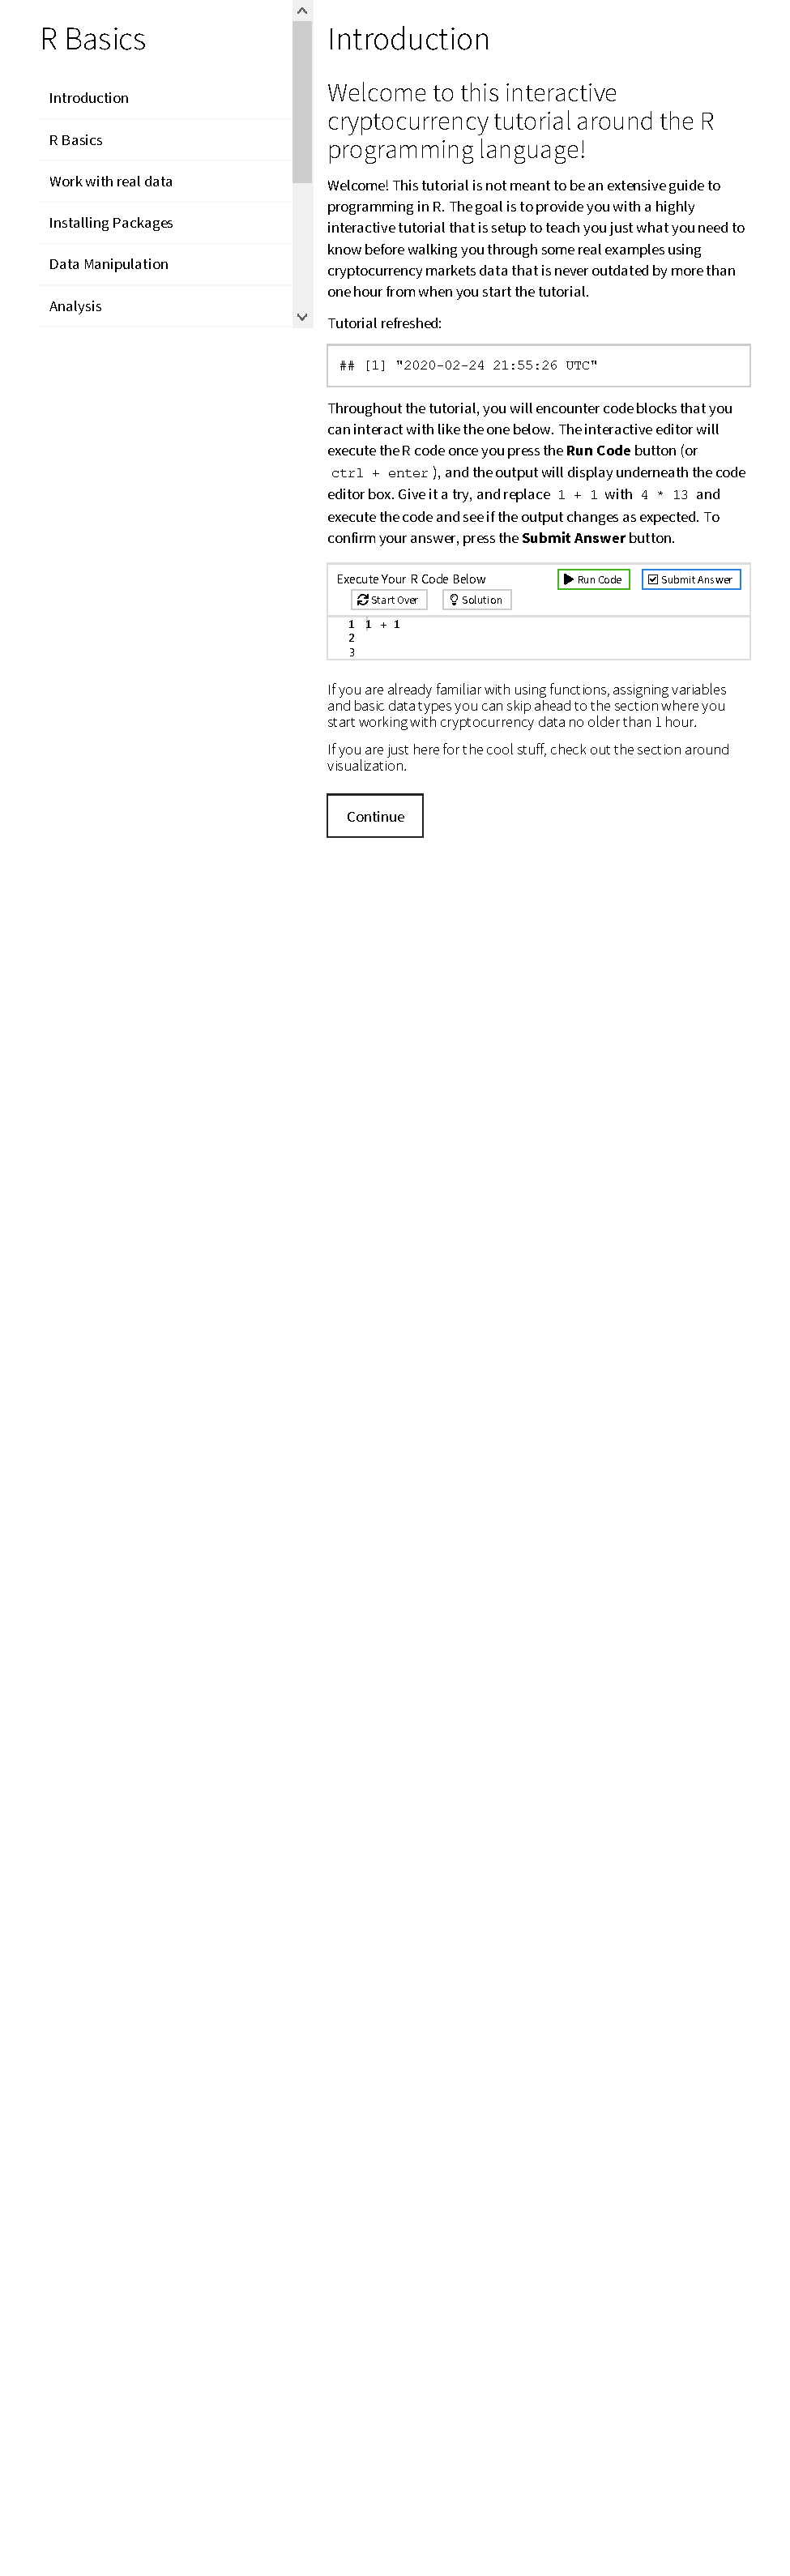
\includegraphics{RStudio-Internship-Application_files/figure-latex/unnamed-chunk-2-1.pdf}}

I would recommend looking at the \textbf{Visualization} section to visually see that the data is never outdated by more than 1 hour.

I post these on my website:
\href{https://predictcrypto.com/tutorials}{
\includegraphics{RStudio-Internship-Application_files/figure-latex/unnamed-chunk-3-1.pdf}}

I'm loving the integrated tutorials tab within RStudio in the 1.3 preview and I am working towards including these with my \texttt{PredictCrypto} package, which I talk more about and use in the \protect\hyperlink{ideal-projects}{next section} of this document.

\hypertarget{bookdown}{%
\subsection{Bookdown}\label{bookdown}}

I was very close to paying for a monthly subscription on gitbook.com because I thought it was such an amazing format to provide documentation through, so I was particularly impressed by and grateful for the bookdown \citep{R-bookdown} package, and these days it's my go to for organizing most things I work on, so why not my application?

This document is obviously an example of a bookdown document in itself, but here's another guide I put together using bookdown:

\href{https://predictcryptodb-quickstart.com/}{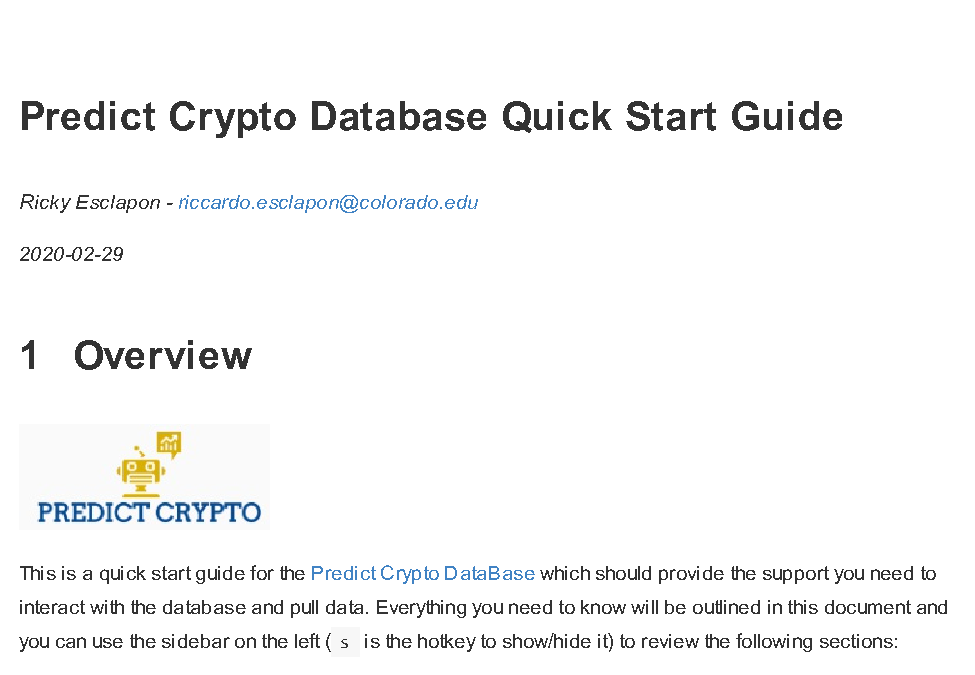
\includegraphics{RStudio-Internship-Application_files/figure-latex/unnamed-chunk-4-1.pdf}}

This guide refreshes daily in order to show a preview of the latest data within the document \href{https://github.com/ries9112/PredictCryptoDB/actions}{and you can look at the GitHub Actions daily runs here}. You can also see the refreshed data in the \href{https://predictcryptodb-quickstart.com/useful-tables.html}{\emph{useful tables} section} of the document.

I also found that documentation done in bookdown can work really great when working within a large company as well, and I put together some very thorough documentation for a project using bookdown that was very well received (but I can't show here). In my particular case it worked really well because I could send the link to the html index of the bookdown document and when opened it would behave like a website hosted on the shared folders within the secure network which ended up being particularly simple and effective.

\hypertarget{presentations}{%
\subsection{Presentations}\label{presentations}}

I am a \textbf{big} fan of ioslides and revealjs in particular as R Markdown outputs. I find the revealjs output to be incredibly cool with the rotating cube animation, and the ability to not only move forward but move downward adds a surprisingly useful tool to break down topics; ioslides is just really clean, well made and easy to use and looks great with widescreen enabled. I aspire to be an expert in Xaringan one day but am not currently.

Making presentations in R Markdown is what really got me working with .Rmd files, because I started working towards a very specific project using an idea I haven't really seen elsewhere of creating presentations that give the user options and as they make their way through the slides, those options affect not only what they see in the slides that come afterwards, but also the options they are given. For example, the user could choose to do an analysis for a particular asset, then choose the main category of the analysis to perform, then the sub-category of the analysis and so on, until by the end of the presentation the user has performed an analysis that was completely unique and tailored to their preferences and interests. See the gif below for an example of what this looks like:

\hypertarget{blogdown}{%
\subsection{Blogdown}\label{blogdown}}

Blogdown\citep{R-blogdown} and bookdown work very similarly, so most of what I mentioned in the \protect\hyperlink{bookdown}{bookdown section} applies here. Because my website predictcrypto.com only shows the latest data based on the current date, I leverage blogdown to create weekly snapshots of the visualizations over the last 7 day period: \url{https://predictcryptoblog.com/}.

\href{https://predictcryptoblog.com/}{\includegraphics{RStudio-Internship-Application_files/figure-latex/unnamed-chunk-5-1.pdf}}

Because all these systems work so well with automation, as I keep adding new interesting content to my website I can also add archives of that content using blogdown.

\hypertarget{pagedown}{%
\subsection{Pagedown}\label{pagedown}}

Pagedown\citep{R-pagedown} is yet another awesome way to create html outputs and I used Nick Strayer's repository \url{https://github.com/nstrayer/cv} to build my cv and resume using his template:

\href{https://ricky-cv.netlify.com/resume}{
\includegraphics{RStudio-Internship-Application_files/figure-latex/unnamed-chunk-6-1.pdf}}

\hypertarget{flexdashboard}{%
\subsection{Flexdashboard}\label{flexdashboard}}

Flexdashboards\citep{R-flexdashboard} were my first introduction to shiny apps and I was completely blown away by that framework and have used it for several projects and is one of my absolute favorite tools.

To get some practice, I converted some of the content found in \href{https://www.tidytextmining.com/}{Tidy Text Mining by Julia Silge and David Robinson} and made it into a flexdashboard. \textbf{I made no changes to the code found within the book}, this was simply an experiment to learn more about flexdashboards and semantic analysis:

\href{https://predictcrypto.shinyapps.io/SemanticAnalysisExample/}{
\includegraphics{RStudio-Internship-Application_files/figure-latex/unnamed-chunk-7-1.pdf}}

\hypertarget{automation}{%
\section{Automation}\label{automation}}

Automation is at the center of everything I do and my one true passion. One of my big goals for RStudio::conf 2020 was to learn more about automating things through GitHub using CI since I always had a hard time figuring that out, and the things I learned about especially relating to GitHub actions and using Netlify were above my expectations in terms of the ease of use, capabilities and free tier offerings, and I am super excited to share how crazy simple automating a very complex process can be through RStudio, GitHub Actions and Netlify. I didn't fnd a huge wealth of information on automating things in R through GitHub Actions and I'm excited to share those learnings in the months to come.

It's pretty mindblowing that these frameworks allow a user to create an interactive book with complex javascript, HTML, CSS, TeX, etc\ldots{} from scratch, deploy it to an https secured website and create an automated process around it, all in less than 10 minutes with minimal code involved. What's even more mindblowing, is that the same methodologies can be applied to make other interfaces, like making a blogdown website, and I can't speak highly enough of all the work Yihui blessed us all with.

I have also done a lot of automation work for \href{https://www.google.com/search?q=vail+resorts+stock}{Vail Resorts} using a tool called \href{https://www.alteryx.com/}{Alteryx} to create fully automated processes with the main purpose of refreshing Tableau dashboards offering refreshed datasets relating to ski pass sales. You can find an example of an automated Alteryx process I created for a personal project doing automated trading on the cryptocurrency markets using my own database, SQL, R and Python here: \url{https://community.alteryx.com/t5/Alteryx-Use-Cases/Predicting-and-Trading-on-the-Cryptocurrency-Markets-using/ta-p/494058}

\hypertarget{rstudio}{%
\section{Fit Within the Company}\label{rstudio}}

I really wanted to go to RStudio::conf 2019 but was not able to make it out and after all the videos got posted I watched most of them and immediately knew I had to come to RStudio::conf 2020 and it was a truly incredible experience.

JJ's talk and BCorp announcement really resonated with me and there is no other company who's mission I agree with more and I would always do my very best in carrying forward those values. I fundamentally believe the most straightforward way to success is to help other people succeed, and I love the values that RStudio holds dear as a company and there is really no other company that I want to work for more than RStudio.

I also work my best remotely and I have a dedicated office to do my work in with a powerful desktop PC and two screens.

\hypertarget{ideal-projects}{%
\chapter{Projects Well Suited For}\label{ideal-projects}}

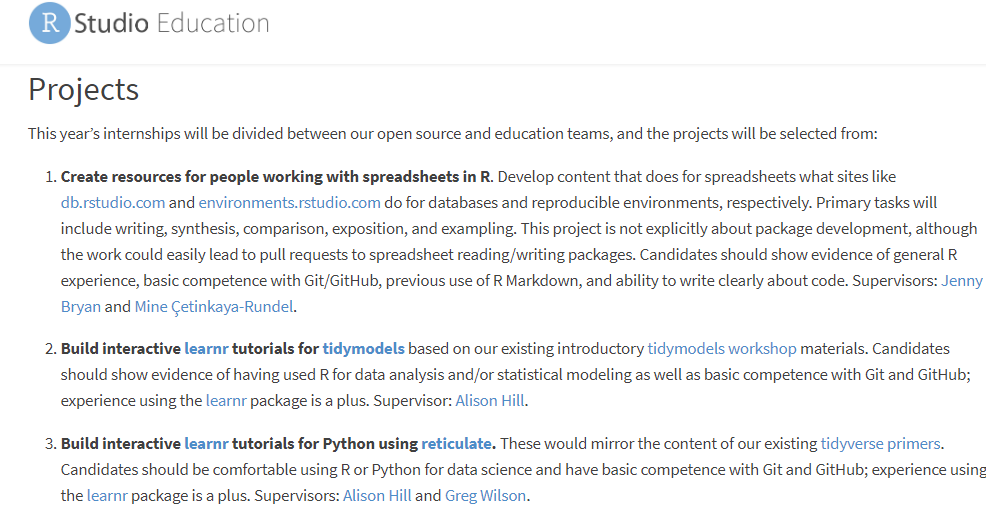
\includegraphics{images/projects_list.png}

\hypertarget{create-resources-for-people-working-with-spreadsheets-in-r}{%
\section{Create resources for people working with spreadsheets in R}\label{create-resources-for-people-working-with-spreadsheets-in-r}}

What better way to show I am suited for a project than to give a hands-on example? See the code below for a use-case using \texttt{googlesheets4}\citep{R-googlesheets4}.

First I will go ahead and import every package in the \texttt{tidyverse}\citep{R-tidyverse}:

\begin{Shaded}
\begin{Highlighting}[]
\KeywordTok{library}\NormalTok{(tidyverse)}
\end{Highlighting}
\end{Shaded}

We will be importing the following spreadsheet:

\begin{Shaded}
\begin{Highlighting}[]
\NormalTok{spreadsheet_url <-}\StringTok{ "https://docs.google.com/spreadsheets/d/1_zRBFrB1au7qhxuDDfDuh_bPLGd6RLrwOL5oQ3sBBX4/edit?usp=sharing"}
\end{Highlighting}
\end{Shaded}

Next let's import the \texttt{googlesheets4} and read a spreadsheet I made for this internship application, specifying the sheet called \emph{coinmetrics\_btc\_eth} inside the function \texttt{read\_sheet()}:

\begin{Shaded}
\begin{Highlighting}[]
\KeywordTok{library}\NormalTok{(googlesheets4)}
\NormalTok{googlesheets_data <-}\StringTok{ }\KeywordTok{read_sheet}\NormalTok{(spreadsheet_url, }\DataTypeTok{sheet =} \StringTok{'coinmetrics_btc_eth'}\NormalTok{) }\OperatorTok\StringTok{ }\KeywordTok{as.data.frame}\NormalTok{()}
\end{Highlighting}
\end{Shaded}

Let's take a peek at the \texttt{datatable()} using \texttt{DT} \citep{R-DT}

\begin{Shaded}
\begin{Highlighting}[]
\KeywordTok{library}\NormalTok{(DT)}
\KeywordTok{datatable}\NormalTok{(googlesheets_data,  }\DataTypeTok{style =} \StringTok{"default"}\NormalTok{, }
          \DataTypeTok{options =} \KeywordTok{list}\NormalTok{(}\DataTypeTok{scrollX =} \OtherTok{TRUE}\NormalTok{, }\DataTypeTok{pageLength=}\DecValTok{5}\NormalTok{,}\DataTypeTok{dom=}\StringTok{'t'}\NormalTok{), }\DataTypeTok{rownames =}\NormalTok{ F)}
\end{Highlighting}
\end{Shaded}

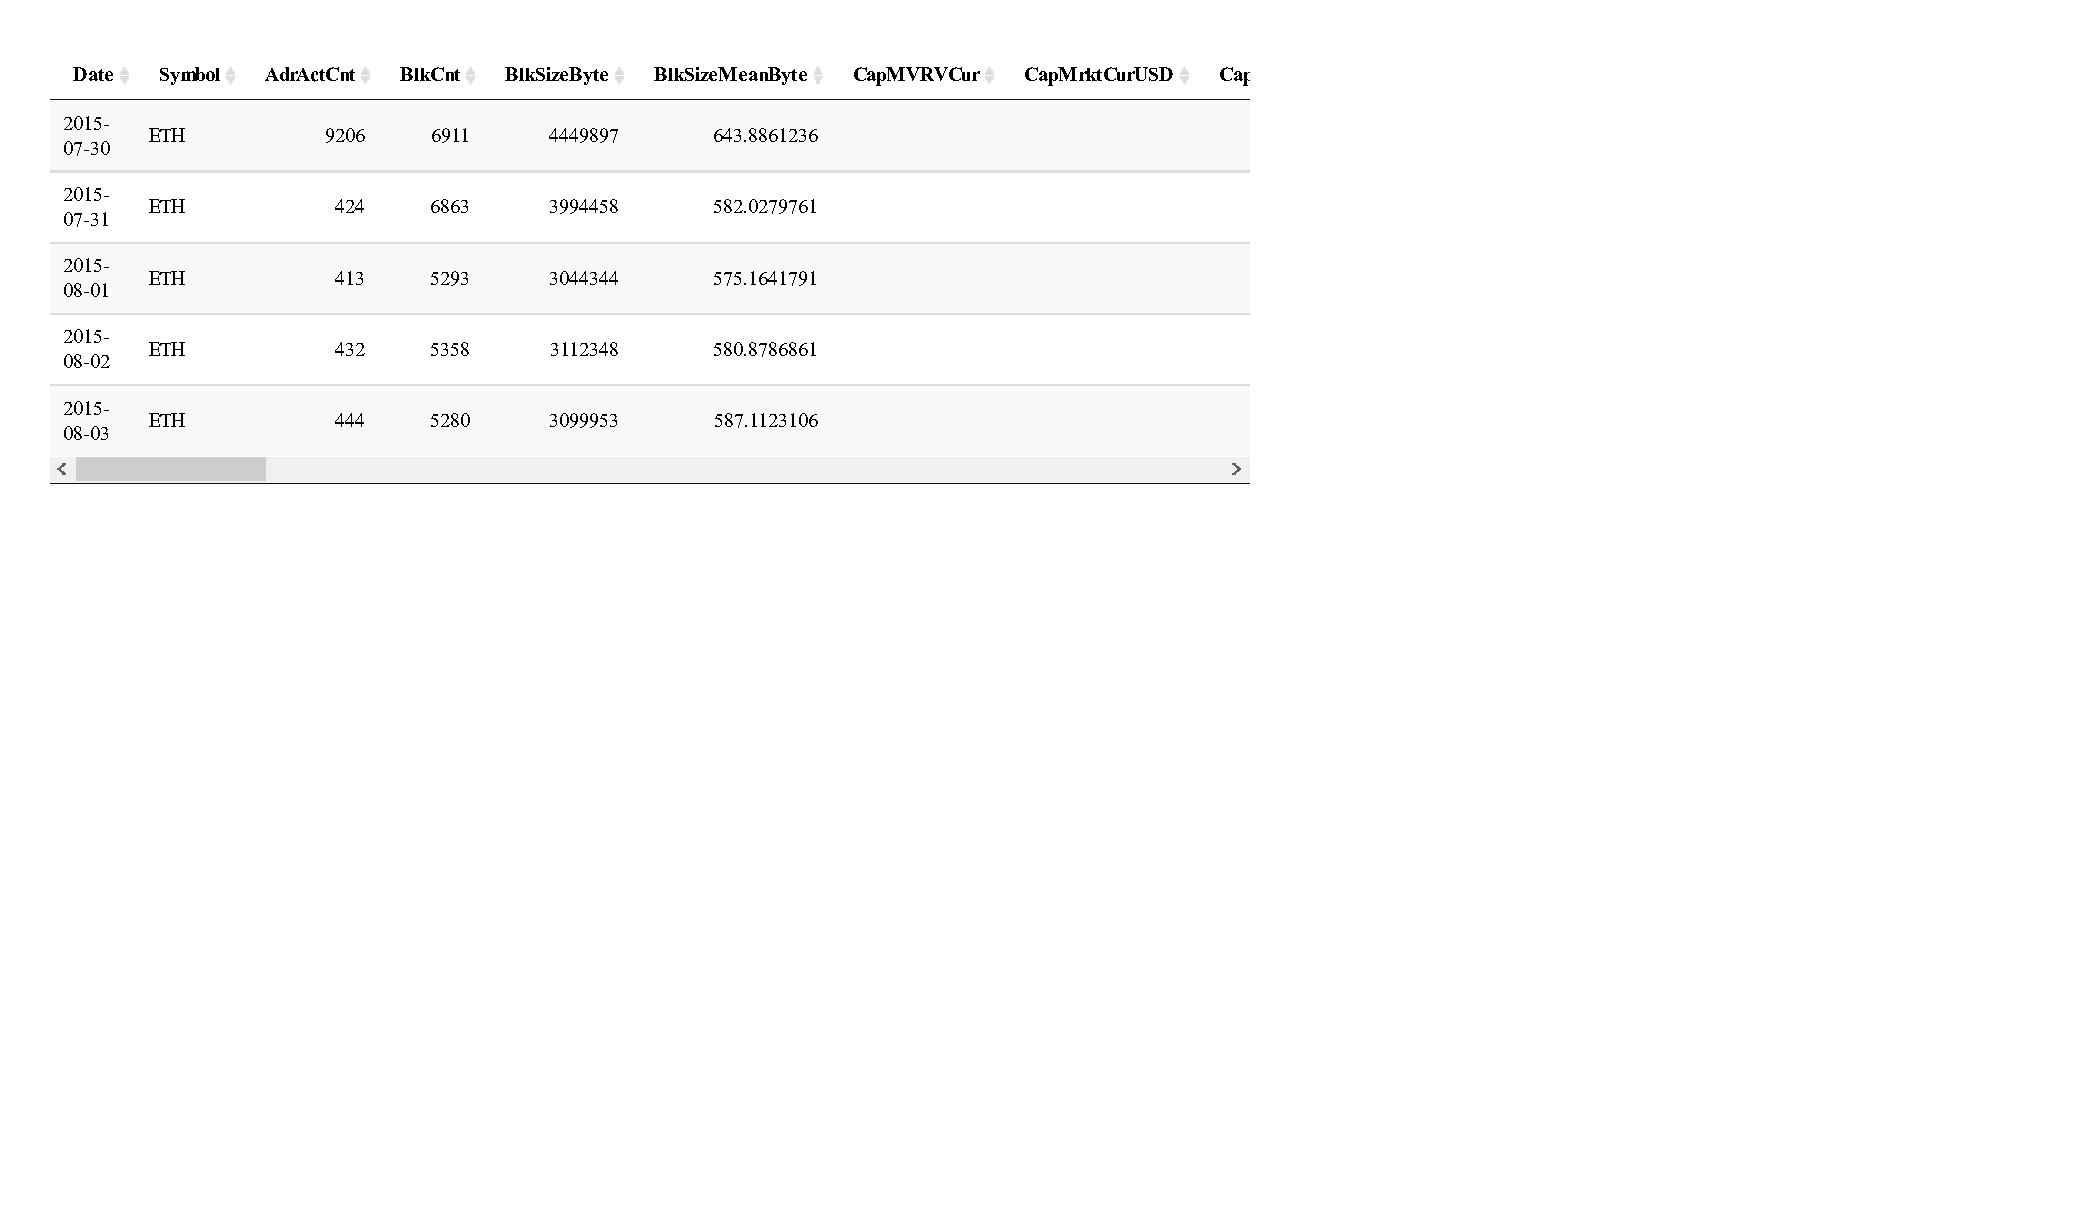
\includegraphics{RStudio-Internship-Application_files/figure-latex/show_googlesheets_data-1.pdf}

\textbf{This data is sourced from the website \href{https://coinmetrics.io/community-network-data/\#comm-files}{coinmetrics.io}}

\href{https://coinmetrics.io/community-data-dictionary/}{Coinmetrics also provides a data dictionary to go along with the data:}

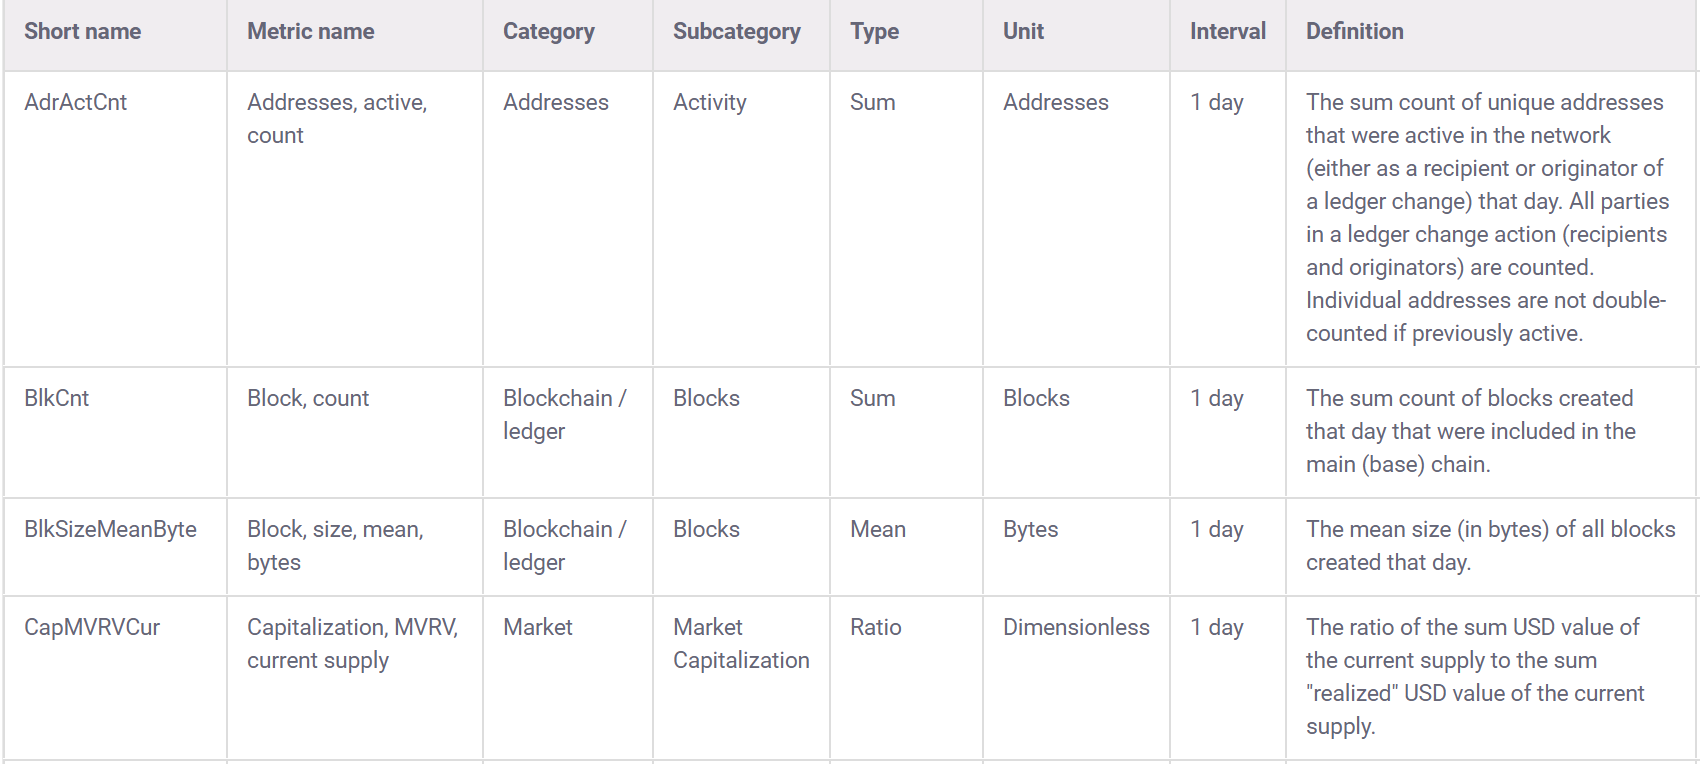
\includegraphics{images/coinmetrics_datadictionary1.png}
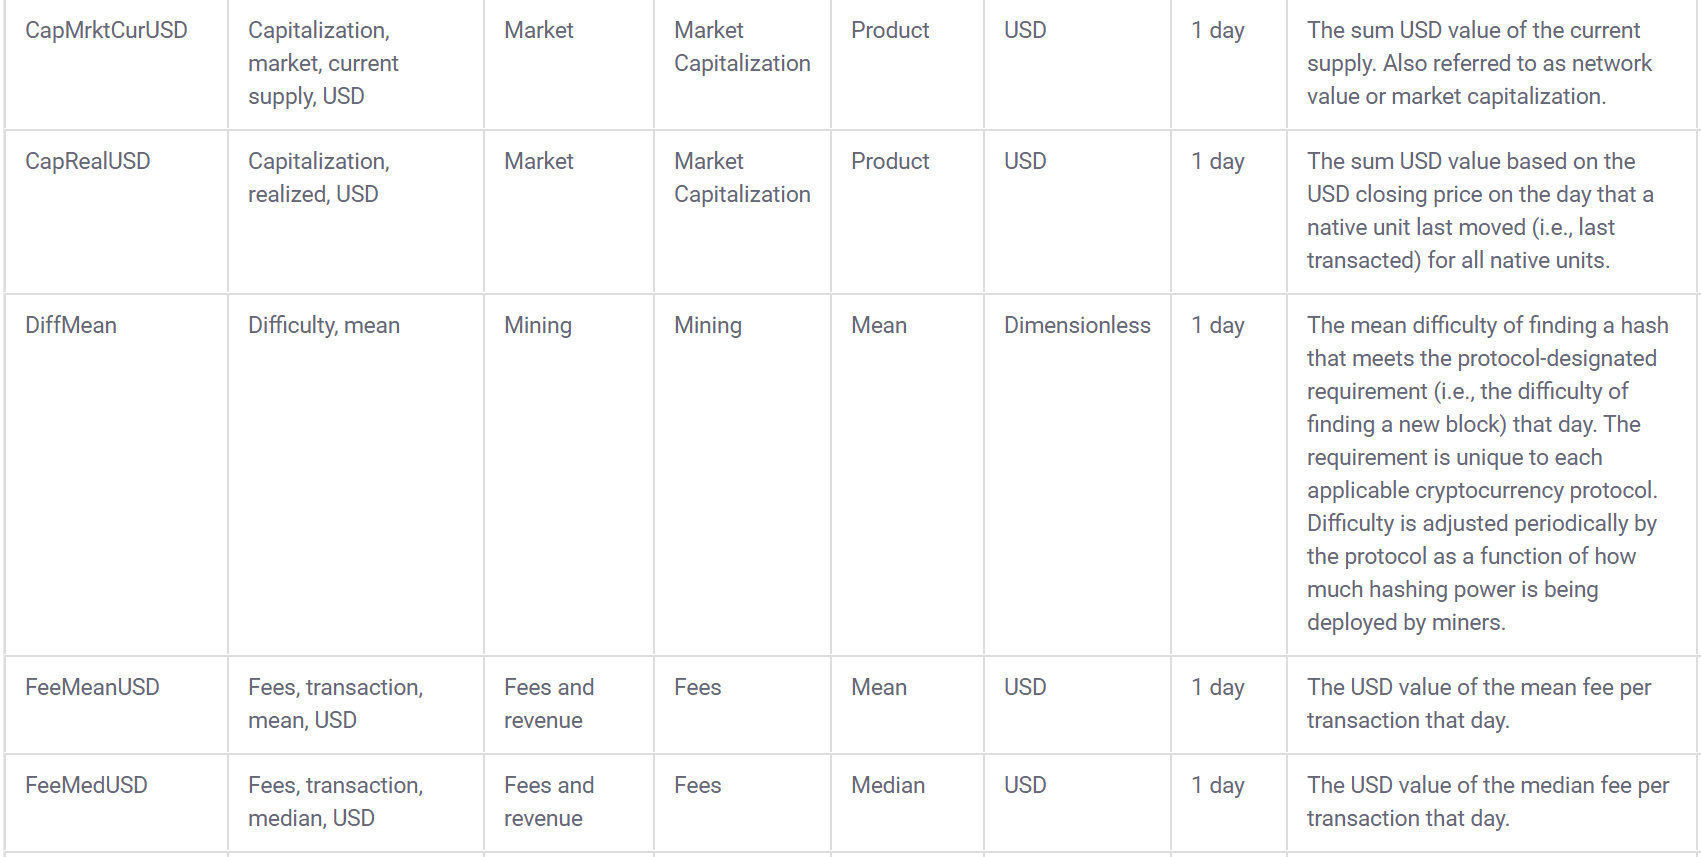
\includegraphics{images/coinmetrics_datadictionary2.png}
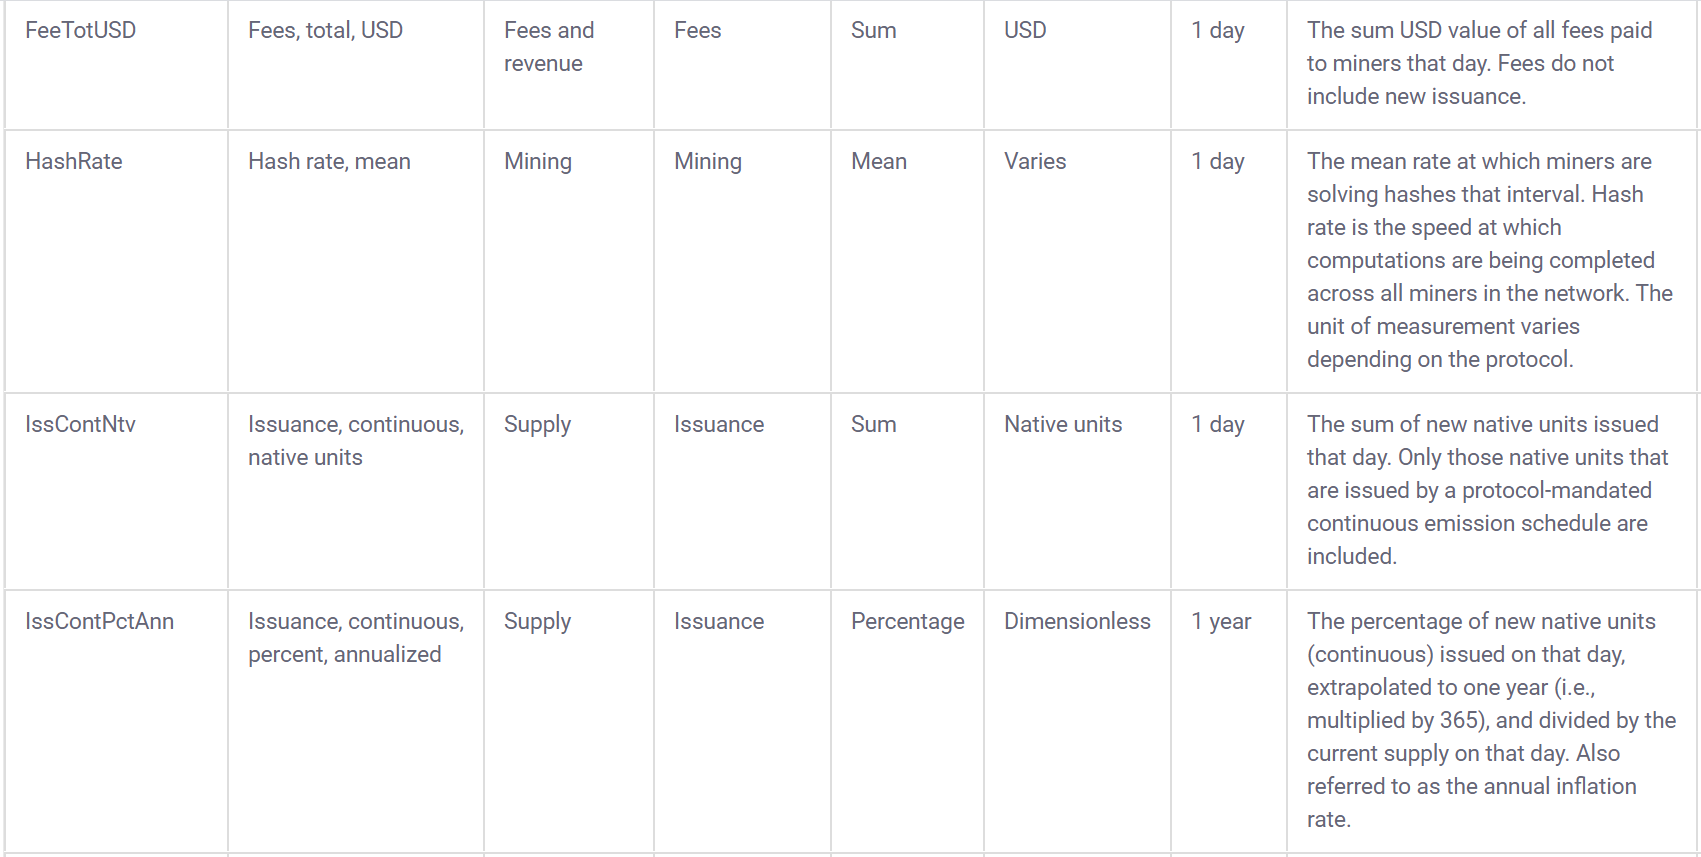
\includegraphics{images/coinmetrics_datadictionary3.png}
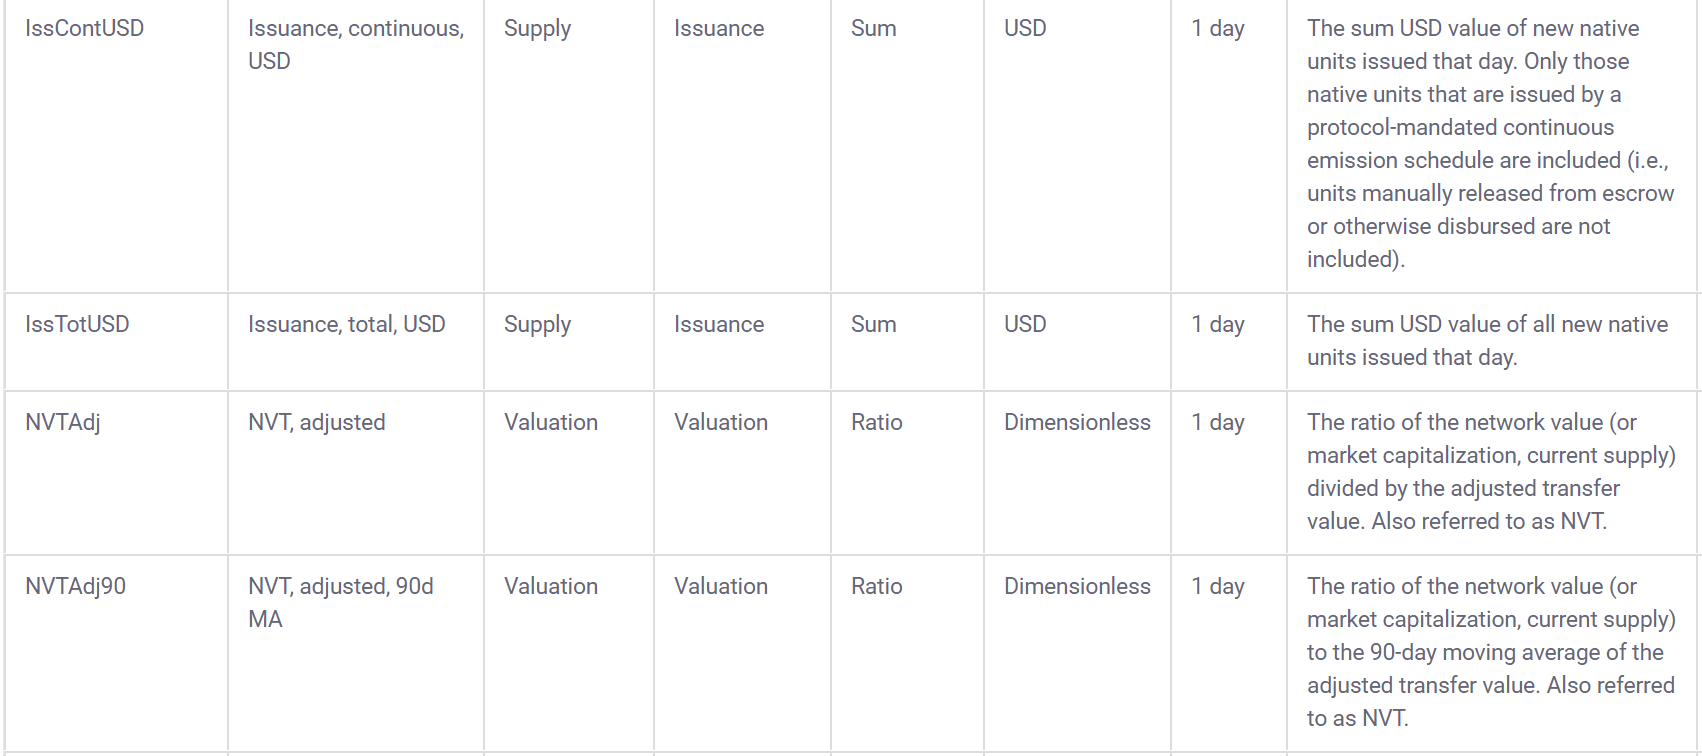
\includegraphics{images/coinmetrics_datadictionary4.png}
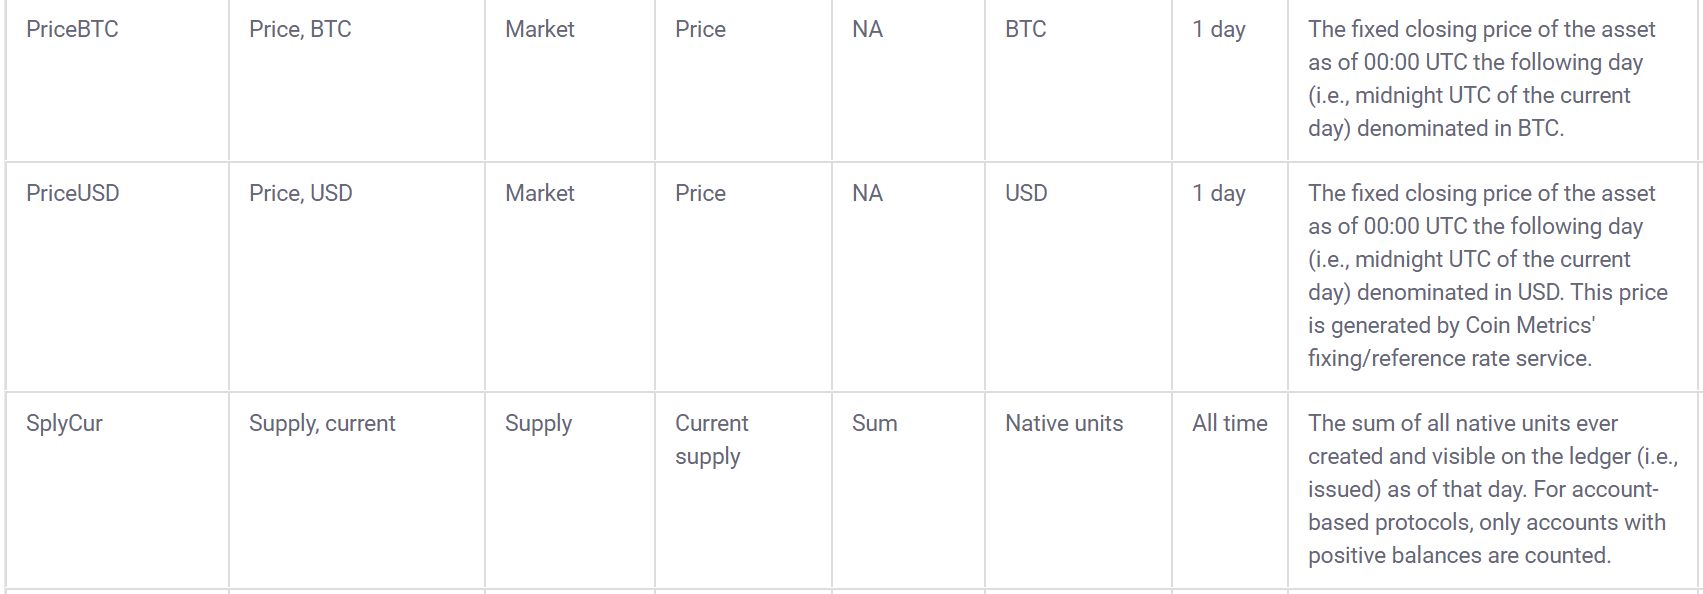
\includegraphics{images/coinmetrics_datadictionary5.png}
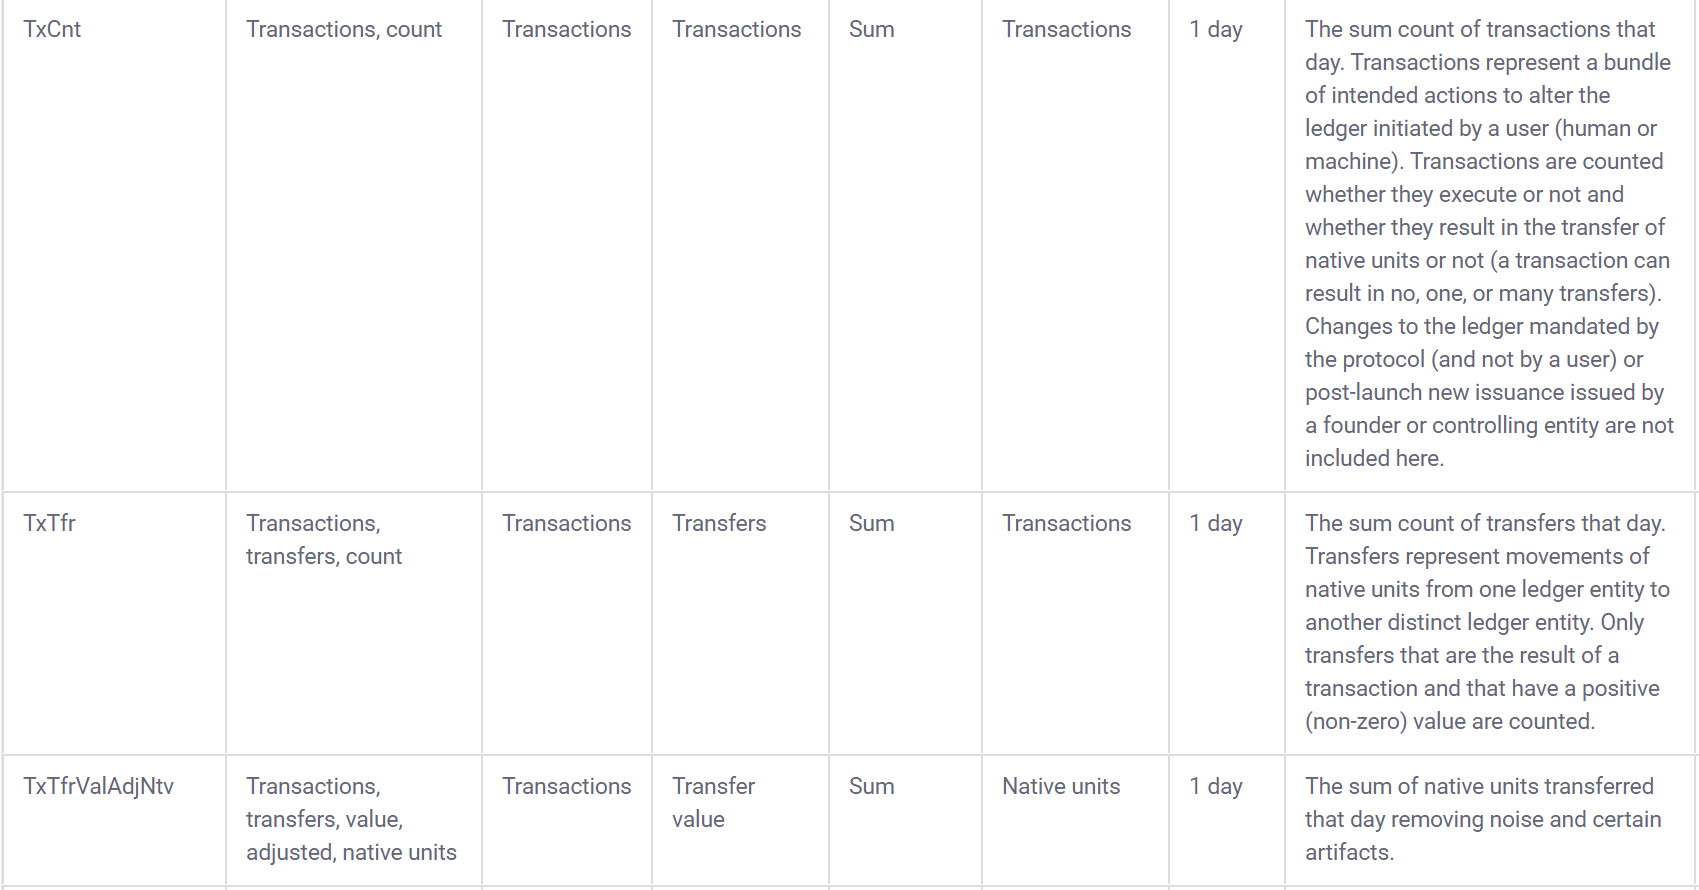
\includegraphics{images/coinmetrics_datadictionary6.png}
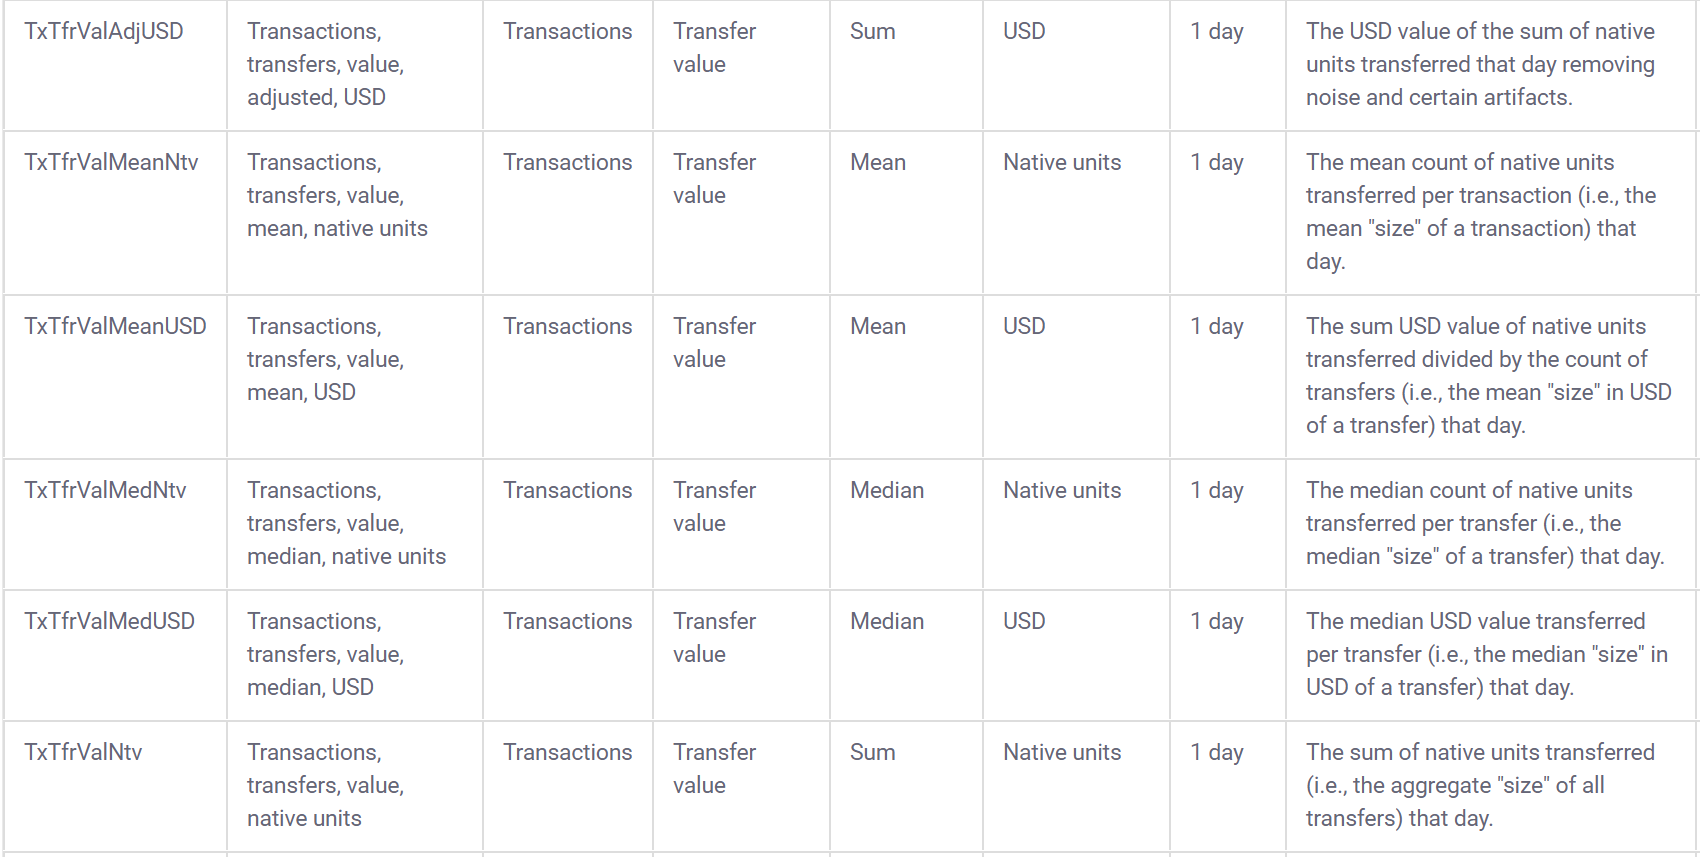
\includegraphics{images/coinmetrics_datadictionary7.png}
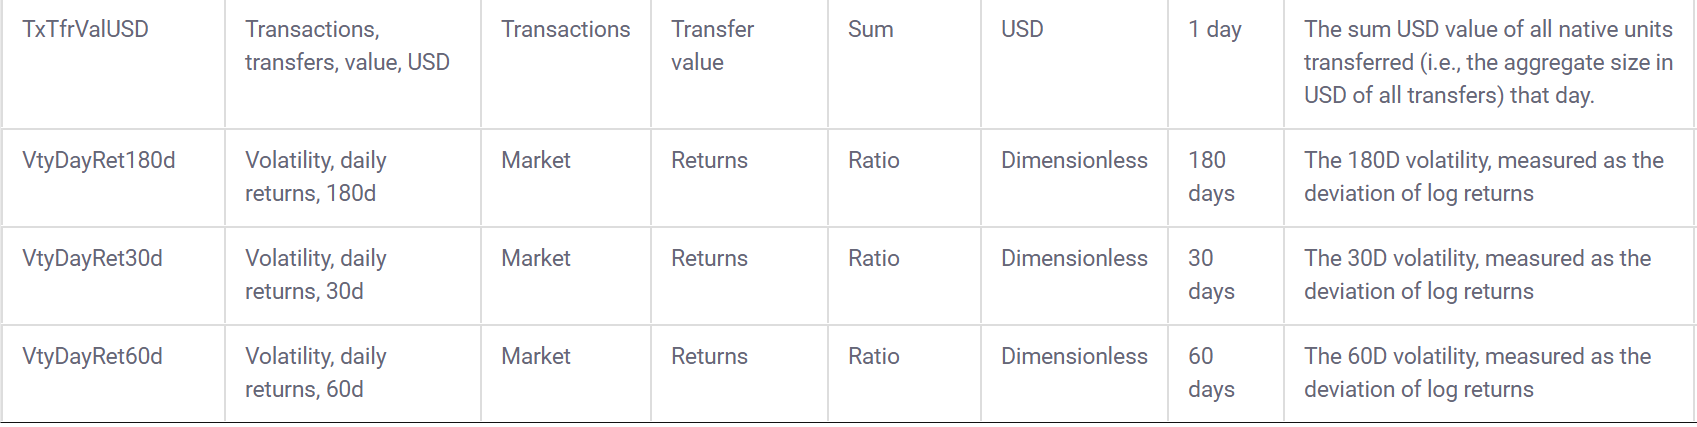
\includegraphics{images/coinmetrics_datadictionary8.png}

\hypertarget{build-interactive-learnr-tutorials-for-tidymodels}{%
\section{Build interactive learnr tutorials for tidymodels}\label{build-interactive-learnr-tutorials-for-tidymodels}}

\hypertarget{data-prep}{%
\subsection{Data Prep}\label{data-prep}}

Using the data from coinmetrics, I will create a predictive model to forecast the percentage change in price over time.

First, I will import a package that I am making that is \textbf{still in development} \texttt{PredictCrypto}:

\begin{Shaded}
\begin{Highlighting}[]
\KeywordTok{library}\NormalTok{(PredictCrypto)}
\end{Highlighting}
\end{Shaded}

(this is an in-development tool that I will use for a research paper I am working on)

I attended the two day building tidy tools workshop working with Charlotte and Hadley at RStudio::conf 2020 and I am comfortable writing packages in R as well as using testthat and showing code coverage for a repository.

Here is the GitHub Pages environment associated with the repository:

\href{https://ries9112.github.io/PredictCrypto/}{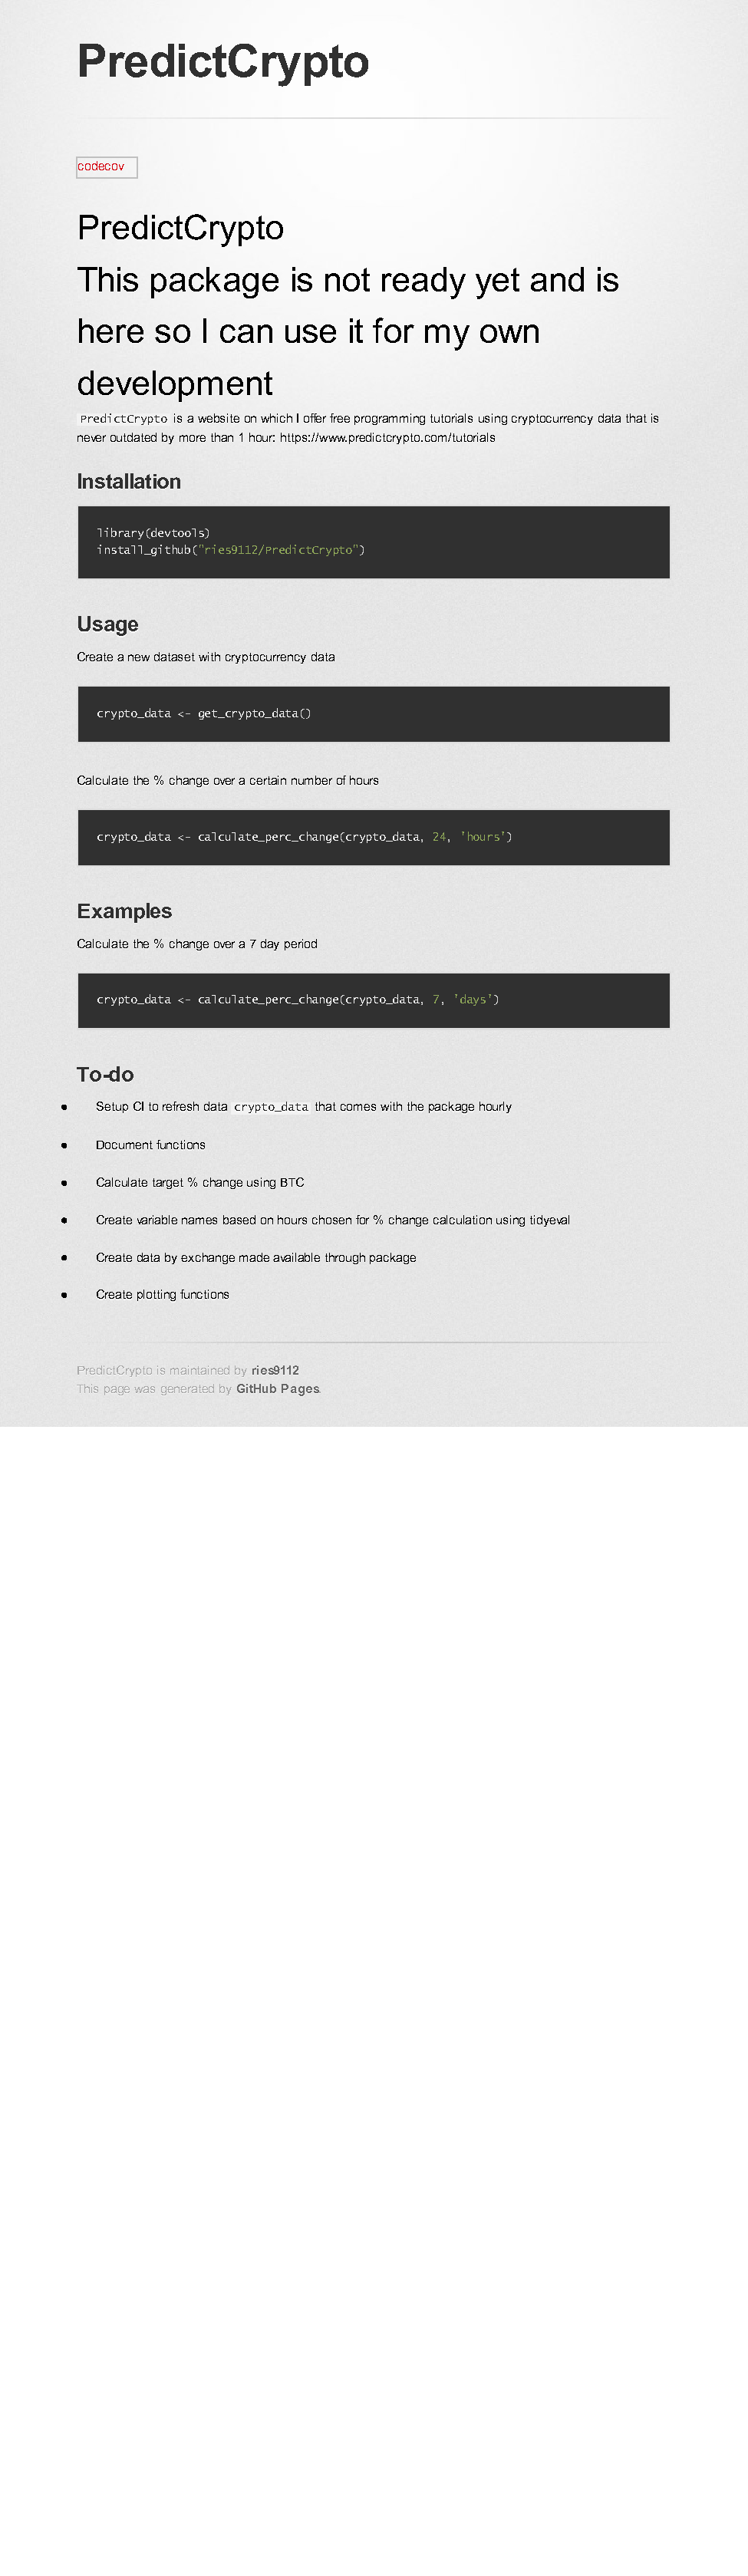
\includegraphics{RStudio-Internship-Application_files/figure-latex/show_github_pages-1.pdf}}

I am going to convert the column names from \textbf{\emph{CamelCase}} to \textbf{\emph{snake\_case}} using the \texttt{janitor}\citep{R-janitor} package because the functions in my package use snake\_case and I want to avoid mixing the two:

Before:

\begin{verbatim}
##  [1] "Date"            "Symbol"          "AdrActCnt"       "BlkCnt"         
##  [5] "BlkSizeByte"     "BlkSizeMeanByte" "CapMVRVCur"      "CapMrktCurUSD"  
##  [9] "CapRealUSD"      "DiffMean"        "FeeMeanNtv"      "FeeMeanUSD"     
## [13] "FeeMedNtv"       "FeeMedUSD"       "FeeTotNtv"       "FeeTotUSD"      
## [17] "HashRate"        "IssContNtv"      "IssContPctAnn"   "IssContUSD"     
## [21] "IssTotNtv"       "IssTotUSD"       "NVTAdj"          "NVTAdj90"       
## [25] "PriceBTC"        "PriceUSD"        "ROI1yr"          "ROI30d"         
## [29] "SplyCur"         "TxCnt"           "TxTfrCnt"        "TxTfrValAdjNtv" 
## [33] "TxTfrValAdjUSD"  "TxTfrValMeanNtv" "TxTfrValMeanUSD" "TxTfrValMedNtv" 
## [37] "TxTfrValMedUSD"  "TxTfrValNtv"     "TxTfrValUSD"     "VtyDayRet180d"  
## [41] "DateTimeUTC"
\end{verbatim}

\begin{Shaded}
\begin{Highlighting}[]
\KeywordTok{library}\NormalTok{(janitor)}
\NormalTok{googlesheets_data <-}\StringTok{ }\KeywordTok{clean_names}\NormalTok{(googlesheets_data)}
\end{Highlighting}
\end{Shaded}

After:

\begin{verbatim}
##  [1] "date"                "symbol"              "adr_act_cnt"        
##  [4] "blk_cnt"             "blk_size_byte"       "blk_size_mean_byte" 
##  [7] "cap_mvrv_cur"        "cap_mrkt_cur_usd"    "cap_real_usd"       
## [10] "diff_mean"           "fee_mean_ntv"        "fee_mean_usd"       
## [13] "fee_med_ntv"         "fee_med_usd"         "fee_tot_ntv"        
## [16] "fee_tot_usd"         "hash_rate"           "iss_cont_ntv"       
## [19] "iss_cont_pct_ann"    "iss_cont_usd"        "iss_tot_ntv"        
## [22] "iss_tot_usd"         "nvt_adj"             "nvt_adj90"          
## [25] "price_btc"           "price_usd"           "roi1yr"             
## [28] "roi30d"              "sply_cur"            "tx_cnt"             
## [31] "tx_tfr_cnt"          "tx_tfr_val_adj_ntv"  "tx_tfr_val_adj_usd" 
## [34] "tx_tfr_val_mean_ntv" "tx_tfr_val_mean_usd" "tx_tfr_val_med_ntv" 
## [37] "tx_tfr_val_med_usd"  "tx_tfr_val_ntv"      "tx_tfr_val_usd"     
## [40] "vty_day_ret180d"     "date_time_utc"
\end{verbatim}

Now that I imported the \texttt{PredictCrypto} package and the data is in snake\_case, I can use the function \texttt{calculate\_percent\_change()} to create the target variable to predict. Before I can do that however, I need one more adjustment to the date/time fields, so let's do that using the \texttt{anytime}\citep{R-anytime} package:

\begin{Shaded}
\begin{Highlighting}[]
\KeywordTok{library}\NormalTok{(anytime)}
\NormalTok{googlesheets_data}\OperatorTok{$}\NormalTok{date <-}\StringTok{ }\KeywordTok{anytime}\NormalTok{(googlesheets_data}\OperatorTok{$}\NormalTok{date)}
\NormalTok{googlesheets_data}\OperatorTok{$}\NormalTok{date_time_utc <-}\StringTok{ }\KeywordTok{anytime}\NormalTok{(googlesheets_data}\OperatorTok{$}\NormalTok{date_time_utc)}
\end{Highlighting}
\end{Shaded}

Now I can use the function \texttt{calculate\_percent\_change()} to calculate the \% change of the price of each cryptocurrency and add a new column \textbf{\emph{target\_percent\_change}} to each row, which will represent the percentage change in price for the 7 day period that came after that data point was collected:

\begin{Shaded}
\begin{Highlighting}[]
\NormalTok{exercise_data <-}\StringTok{ }\NormalTok{PredictCrypto}\OperatorTok{::}\KeywordTok{calculate_percent_change}\NormalTok{(googlesheets_data, }\DecValTok{7}\NormalTok{, }\StringTok{'days'}\NormalTok{)}
\end{Highlighting}
\end{Shaded}

Let's take a peek at the new field:

\begin{Shaded}
\begin{Highlighting}[]
\KeywordTok{tail}\NormalTok{(exercise_data}\OperatorTok{$}\NormalTok{target_percent_change, }\DecValTok{10}\NormalTok{)}
\end{Highlighting}
\end{Shaded}

\begin{verbatim}
##  [1]   2.371123   7.142857  20.891949  23.846718   6.707045  19.548486
##  [7] -25.610849 -21.561229 -30.693069 -41.121855
\end{verbatim}

I could easily change this to a 14 day period:

\begin{Shaded}
\begin{Highlighting}[]
\KeywordTok{calculate_percent_change}\NormalTok{(googlesheets_data, }\DecValTok{14}\NormalTok{, }\StringTok{'days'}\NormalTok{) }\OperatorTok\StringTok{ }\KeywordTok{tail}\NormalTok{(}\DecValTok{10}\NormalTok{) }\OperatorTok\StringTok{ }\KeywordTok{select}\NormalTok{(target_percent_change)}
\end{Highlighting}
\end{Shaded}

\begin{verbatim}
##      target_percent_change
## 5104             18.281533
## 5105             25.714286
## 5106             20.496231
## 5107              8.184818
## 5108              1.779083
## 5109              4.327005
## 5110            -28.003738
## 5111            -19.701349
## 5112            -25.742574
## 5113            -28.821062
\end{verbatim}

Or a 24 hour period:

\begin{Shaded}
\begin{Highlighting}[]
\KeywordTok{calculate_percent_change}\NormalTok{(googlesheets_data, }\DecValTok{24}\NormalTok{, }\StringTok{'hours'}\NormalTok{) }\OperatorTok\StringTok{ }\KeywordTok{tail}\NormalTok{(}\DecValTok{10}\NormalTok{) }\OperatorTok\StringTok{ }\KeywordTok{select}\NormalTok{(target_percent_change)}
\end{Highlighting}
\end{Shaded}

\begin{verbatim}
##      target_percent_change
## 5130              0.492989
## 5131              4.682143
## 5132             10.801132
## 5133             -7.332233
## 5134             -9.989603
## 5135              3.630922
## 5136            -26.167717
## 5137              5.963659
## 5138             -7.504950
## 5139             -5.871389
\end{verbatim}

\textbf{\emph{Disclaimer:}} \textbf{Most of the code to follow was built using the content made available by Allison Hill from the RStudio::conf2020 intro to machine learning workshop and was not code I was familiar with before writing it for this internship application:}

\url{https://education.rstudio.com/blog/2020/02/conf20-intro-ml/}

\url{https://conf20-intro-ml.netlify.com/materials/01-predicting/}

\hypertarget{feature-scaling}{%
\subsection{Feature scaling}\label{feature-scaling}}

Before getting started on the predictive modeling section, it's a good idea for us to scale the numeric data in our dataset. Some of the fields in the dataset are bound to have dramatically different ranges in their values:

\begin{Shaded}
\begin{Highlighting}[]
\KeywordTok{mean}\NormalTok{(exercise_data}\OperatorTok{$}\NormalTok{roi_}\DecValTok{30}\NormalTok{_days)}
\end{Highlighting}
\end{Shaded}

\begin{verbatim}
## Warning in mean.default(exercise_data$roi_30_days): argument is not numeric or
## logical: returning NA
\end{verbatim}

\begin{verbatim}
## [1] NA
\end{verbatim}

\begin{Shaded}
\begin{Highlighting}[]
\KeywordTok{mean}\NormalTok{(exercise_data}\OperatorTok{$}\NormalTok{supply_current)}
\end{Highlighting}
\end{Shaded}

\begin{verbatim}
## Warning in mean.default(exercise_data$supply_current): argument is not numeric
## or logical: returning NA
\end{verbatim}

\begin{verbatim}
## [1] NA
\end{verbatim}

This can be problematic for some models (not every model has this issue), and the difference in the magnitude of the numbers could unfairly influence the model to think that the variable with the larger numbers is more statistically important than the one with the lesser values when that might not actually be true.

For feature scaling, we need to do two things:

\begin{enumerate}
\def\labelenumi{\arabic{enumi}.}
\item
  \textbf{\emph{Center}} the data in every column to have a mean of zero
\item
  \textbf{\emph{Scale}} the data in every column to have a standard deviation of one
\end{enumerate}

The \texttt{recipes} \citep{R-recipes} package is a very useful package for pre-processing data before doing predictive modeling, and it allows us to center the way we do our data engineering around the independent variable we are looking to predict, which in our case is the \texttt{target\_percent\_change}. We can make a recipe which centers all numeric fields in the data using \texttt{step\_center()} and then scale them using \texttt{step\_scale()}:

\begin{Shaded}
\begin{Highlighting}[]
\KeywordTok{library}\NormalTok{(recipes)}
\NormalTok{scaling_recipe <-}\StringTok{ }\KeywordTok{recipe}\NormalTok{(target_percent_change }\OperatorTok{~}\StringTok{ }\NormalTok{., }\DataTypeTok{data =}\NormalTok{ exercise_data) }\OperatorTok
\StringTok{  }\KeywordTok{step_center}\NormalTok{(}\KeywordTok{all_numeric}\NormalTok{()) }\OperatorTok\StringTok{ }
\StringTok{  }\KeywordTok{step_scale}\NormalTok{(}\KeywordTok{all_numeric}\NormalTok{())}
\end{Highlighting}
\end{Shaded}

Now that we have made a data pre-processing \emph{recipe}, let's map it to the \texttt{exercise\_data} dataset:

\begin{Shaded}
\begin{Highlighting}[]
\NormalTok{crypto_data_scaled <-}\StringTok{ }\NormalTok{scaling_recipe }\OperatorTok\StringTok{ }\KeywordTok{prep}\NormalTok{(exercise_data) }
\NormalTok{crypto_data_scaled}
\end{Highlighting}
\end{Shaded}

\begin{verbatim}
## Data Recipe
## 
## Inputs:
## 
##       role #variables
##    outcome          1
##  predictor         46
## 
## Training data contained 5127 data points and 700 incomplete rows. 
## 
## Operations:
## 
## Centering for adr_act_cnt, blk_cnt, ... [trained]
## Scaling for adr_act_cnt, blk_cnt, ... [trained]
\end{verbatim}

Now let's use \texttt{bake()} to put the old dataset in the oven and get back the scaled data 🍰:

\begin{Shaded}
\begin{Highlighting}[]
\NormalTok{crypto_data_scaled <-}\StringTok{ }\NormalTok{crypto_data_scaled }\OperatorTok\StringTok{ }\KeywordTok{bake}\NormalTok{(exercise_data)}
\end{Highlighting}
\end{Shaded}

Now the values are scaled:

\begin{Shaded}
\begin{Highlighting}[]
\KeywordTok{head}\NormalTok{(crypto_data_scaled}\OperatorTok{$}\NormalTok{active_addresses,}\DecValTok{5}\NormalTok{)}
\end{Highlighting}
\end{Shaded}

\begin{verbatim}
## Warning: Unknown or uninitialised column: 'active_addresses'.
\end{verbatim}

\begin{verbatim}
## NULL
\end{verbatim}

You can see the difference from the previous values:

\begin{Shaded}
\begin{Highlighting}[]
\KeywordTok{head}\NormalTok{(exercise_data}\OperatorTok{$}\NormalTok{active_addresses,}\DecValTok{5}\NormalTok{)}
\end{Highlighting}
\end{Shaded}

\begin{verbatim}
## NULL
\end{verbatim}

\hypertarget{predictive-modeling}{%
\subsection{Predictive Modeling}\label{predictive-modeling}}

Create the \texttt{parsnip} \citep{R-parsnip} model

\begin{Shaded}
\begin{Highlighting}[]
\KeywordTok{library}\NormalTok{(parsnip)}
\NormalTok{lm_model <-}\StringTok{ }\KeywordTok{linear_reg}\NormalTok{() }\OperatorTok\StringTok{              }
\StringTok{  }\KeywordTok{set_engine}\NormalTok{(}\StringTok{"lm"}\NormalTok{) }\OperatorTok\StringTok{             }
\StringTok{  }\KeywordTok{set_mode}\NormalTok{(}\StringTok{"regression"}\NormalTok{)}
\end{Highlighting}
\end{Shaded}

List of models to refer to: \url{https://tidymodels.github.io/parsnip/articles/articles/Models.html}

Random Forest:

\begin{Shaded}
\begin{Highlighting}[]
\NormalTok{random_forest_model <-}\StringTok{ }\KeywordTok{rand_forest}\NormalTok{(}\DataTypeTok{trees =} \DecValTok{100}\NormalTok{, }\DataTypeTok{mode =} \StringTok{"regression"}\NormalTok{) }\OperatorTok
\StringTok{  }\KeywordTok{set_engine}\NormalTok{(}\StringTok{"randomForest"}\NormalTok{) }
\end{Highlighting}
\end{Shaded}

XGBoost:

\begin{Shaded}
\begin{Highlighting}[]
\NormalTok{xgboost_model <-}\StringTok{ }\NormalTok{xgboost_parsnip <-}\StringTok{ }\KeywordTok{boost_tree}\NormalTok{() }\OperatorTok\StringTok{ }
\StringTok{  }\KeywordTok{set_engine}\NormalTok{(}\StringTok{"xgboost"}\NormalTok{) }\OperatorTok\StringTok{             }
\StringTok{  }\KeywordTok{set_mode}\NormalTok{(}\StringTok{"regression"}\NormalTok{)}
\end{Highlighting}
\end{Shaded}

Remove fields not used for models (NOTE: REMOVE price\_usd\_x\_daysLater AND date\_time\_x\_days\_Later FROM BEING GENERATED INSIDE THE FUNCTION)

\begin{Shaded}
\begin{Highlighting}[]
\NormalTok{exercise_data <-}\StringTok{ }\KeywordTok{select}\NormalTok{(exercise_data, }\OperatorTok{-}\NormalTok{date_time_utc, }\OperatorTok{-}\NormalTok{date_time, }\OperatorTok{-}\NormalTok{pkDummy, }\OperatorTok{-}\NormalTok{pkey, }\OperatorTok{-}\NormalTok{price_usd_x_daysLater, }\OperatorTok{-}\NormalTok{date_time_x_daysLater)}
\end{Highlighting}
\end{Shaded}

Create train/test split using \texttt{rsample}\citep{R-rsample}:

(should I do 10-fold cross validation?)

\begin{Shaded}
\begin{Highlighting}[]
\KeywordTok{library}\NormalTok{(rsample)}

\KeywordTok{set.seed}\NormalTok{(}\DecValTok{250}\NormalTok{)}
\NormalTok{crypto_data <-}\StringTok{ }\KeywordTok{initial_split}\NormalTok{(exercise_data, }\DataTypeTok{prop =} \FloatTok{0.8}\NormalTok{)}
\NormalTok{crypto_train <-}\StringTok{ }\KeywordTok{training}\NormalTok{(crypto_data)}
\NormalTok{crypto_test  <-}\StringTok{  }\KeywordTok{testing}\NormalTok{(crypto_data)}
\end{Highlighting}
\end{Shaded}

\hypertarget{trainfit-the-model}{%
\subsection{Train/fit the model:}\label{trainfit-the-model}}

\begin{Shaded}
\begin{Highlighting}[]
\KeywordTok{library}\NormalTok{(modelr)}
\NormalTok{lm_fitted <-}\StringTok{ }\NormalTok{lm_model }\OperatorTok\StringTok{ }\KeywordTok{fit}\NormalTok{(price_usd }\OperatorTok{~}\StringTok{ }\NormalTok{., }\DataTypeTok{data=}\NormalTok{crypto_train)}
\end{Highlighting}
\end{Shaded}

Random Forest:

\begin{Shaded}
\begin{Highlighting}[]
\NormalTok{random_forest_fitted <-}\StringTok{ }\NormalTok{random_forest_model }\OperatorTok
\StringTok{  }\KeywordTok{fit}\NormalTok{(target_percent_change }\OperatorTok{~}\StringTok{ }\NormalTok{., }\DataTypeTok{data =}\NormalTok{ exercise_data)}
\end{Highlighting}
\end{Shaded}

XGBoost:

\begin{Shaded}
\begin{Highlighting}[]
\NormalTok{xgboost_fitted <-}\StringTok{ }\NormalTok{xgboost_model }\OperatorTok\StringTok{ }\KeywordTok{fit}\NormalTok{(price_usd }\OperatorTok{~}\StringTok{ }\NormalTok{., }\DataTypeTok{data=}\NormalTok{crypto_train)}
\end{Highlighting}
\end{Shaded}

Use the trained model to make predictions on test data:

\begin{Shaded}
\begin{Highlighting}[]
\KeywordTok{library}\NormalTok{(tidymodels)}
\NormalTok{lm_predictions <-}\StringTok{ }\NormalTok{lm_fitted }\OperatorTok\StringTok{ }\KeywordTok{predict}\NormalTok{(crypto_test)}
\end{Highlighting}
\end{Shaded}

\begin{Shaded}
\begin{Highlighting}[]
\NormalTok{xgboost_predictions <-}\StringTok{ }\NormalTok{xgboost_fitted }\OperatorTok\StringTok{ }\KeywordTok{predict}\NormalTok{(crypto_test)}
\end{Highlighting}
\end{Shaded}

Join the full dataset back to the predictions:

\begin{Shaded}
\begin{Highlighting}[]
\NormalTok{lm_predictions <-}\StringTok{ }\NormalTok{lm_predictions }\OperatorTok\StringTok{ }\KeywordTok{bind_cols}\NormalTok{(crypto_test)}

\NormalTok{xgboost_predictions <-}\StringTok{ }\NormalTok{xgboost_predictions }\OperatorTok\StringTok{ }\KeywordTok{bind_cols}\NormalTok{(crypto_test)}
\end{Highlighting}
\end{Shaded}

Get metrics:

\begin{Shaded}
\begin{Highlighting}[]
\NormalTok{lm_predictions }\OperatorTok
\StringTok{  }\KeywordTok{metrics}\NormalTok{(}\DataTypeTok{truth =}\NormalTok{ target_percent_change, }\DataTypeTok{estimate =}\NormalTok{ .pred)}
\end{Highlighting}
\end{Shaded}

\begin{verbatim}
## # A tibble: 3 x 3
##   .metric .estimator   .estimate
##   <chr>   <chr>            <dbl>
## 1 rmse    standard   3580.      
## 2 rsq     standard      0.000277
## 3 mae     standard   1749.
\end{verbatim}

\begin{Shaded}
\begin{Highlighting}[]
\NormalTok{xgboost_predictions }\OperatorTok
\StringTok{  }\KeywordTok{metrics}\NormalTok{(}\DataTypeTok{truth =}\NormalTok{ target_percent_change, }\DataTypeTok{estimate =}\NormalTok{ .pred)}
\end{Highlighting}
\end{Shaded}

\begin{verbatim}
## # A tibble: 3 x 3
##   .metric .estimator   .estimate
##   <chr>   <chr>            <dbl>
## 1 rmse    standard   3316.      
## 2 rsq     standard      0.000975
## 3 mae     standard   1496.
\end{verbatim}

\hypertarget{now-make-one-model-for-each-cryptocurrency.}{%
\subsection{Now make one model for each cryptocurrency.}\label{now-make-one-model-for-each-cryptocurrency.}}

\textbf{\emph{Code adapted from: \url{https://r4ds.had.co.nz/many-models.html}}}

First I group the data

\begin{Shaded}
\begin{Highlighting}[]
\NormalTok{crypto_data_grouped <-}\StringTok{ }\NormalTok{exercise_data }\OperatorTok\StringTok{ }\KeywordTok{group_by}\NormalTok{(symbol) }\OperatorTok\StringTok{ }\KeywordTok{nest}\NormalTok{()}
\end{Highlighting}
\end{Shaded}

\begin{Shaded}
\begin{Highlighting}[]
\NormalTok{crypto_data_grouped}
\end{Highlighting}
\end{Shaded}

\begin{verbatim}
## # A tibble: 2 x 2
## # Groups:   symbol [2]
##   symbol data                 
##   <chr>  <list>               
## 1 BTC    <tibble [3,502 x 40]>
## 2 ETH    <tibble [1,625 x 40]>
\end{verbatim}

Make a helper function with the model:

\begin{Shaded}
\begin{Highlighting}[]
\NormalTok{grouped_linear_model <-}\StringTok{ }\ControlFlowTok{function}\NormalTok{(df) \{}
  \KeywordTok{lm}\NormalTok{(target_percent_change }\OperatorTok{~}\StringTok{ }\NormalTok{., }\DataTypeTok{data =}\NormalTok{ df)}
\NormalTok{\}}
\end{Highlighting}
\end{Shaded}

Now we can use \texttt{purrr}\citep{R-purrr} to apply the model to each element of the grouped dataframe:

\begin{Shaded}
\begin{Highlighting}[]
\NormalTok{grouped_models <-}\StringTok{ }\KeywordTok{map}\NormalTok{(crypto_data_grouped}\OperatorTok{$}\NormalTok{data, grouped_linear_model)}
\end{Highlighting}
\end{Shaded}

The models can be added into the dataframe as nested lists. We can also add the corresponding residuals:

\begin{Shaded}
\begin{Highlighting}[]
\NormalTok{crypto_data_grouped <-}\StringTok{ }\NormalTok{crypto_data_grouped }\OperatorTok\StringTok{ }
\StringTok{  }\KeywordTok{mutate}\NormalTok{(}\DataTypeTok{model=}\KeywordTok{map}\NormalTok{(data,grouped_linear_model)) }\OperatorTok\StringTok{ }
\StringTok{  }\KeywordTok{mutate}\NormalTok{(}\DataTypeTok{resids =} \KeywordTok{map2}\NormalTok{(data, model, add_residuals))}
\end{Highlighting}
\end{Shaded}

Let's look at the object again:

\begin{Shaded}
\begin{Highlighting}[]
\NormalTok{crypto_data_grouped}
\end{Highlighting}
\end{Shaded}

\begin{verbatim}
## # A tibble: 2 x 4
## # Groups:   symbol [2]
##   symbol data                  model  resids               
##   <chr>  <list>                <list> <list>               
## 1 BTC    <tibble [3,502 x 40]> <lm>   <tibble [3,502 x 41]>
## 2 ETH    <tibble [1,625 x 40]> <lm>   <tibble [1,625 x 41]>
\end{verbatim}

Let's unnest the residuals to take a closer look:

\begin{Shaded}
\begin{Highlighting}[]
\NormalTok{resids <-}\StringTok{ }\KeywordTok{unnest}\NormalTok{(crypto_data_grouped, resids)}
\end{Highlighting}
\end{Shaded}

\begin{Shaded}
\begin{Highlighting}[]
\NormalTok{resids }\OperatorTok\StringTok{ }
\StringTok{  }\KeywordTok{ggplot}\NormalTok{(}\KeywordTok{aes}\NormalTok{(date, resid)) }\OperatorTok{+}
\StringTok{    }\KeywordTok{geom_line}\NormalTok{(}\KeywordTok{aes}\NormalTok{(}\DataTypeTok{group =}\NormalTok{ symbol), }\DataTypeTok{alpha =} \DecValTok{1} \OperatorTok{/}\StringTok{ }\DecValTok{3}\NormalTok{) }\OperatorTok{+}\StringTok{ }
\StringTok{    }\KeywordTok{geom_smooth}\NormalTok{(}\DataTypeTok{se =} \OtherTok{FALSE}\NormalTok{) }\OperatorTok{+}
\StringTok{    }\KeywordTok{ylim}\NormalTok{(}\KeywordTok{c}\NormalTok{(}\OperatorTok{-}\DecValTok{20}\NormalTok{,}\DecValTok{20}\NormalTok{)) }\OperatorTok{+}
\StringTok{    }\KeywordTok{facet_wrap}\NormalTok{(}\OperatorTok{~}\NormalTok{symbol)}
\end{Highlighting}
\end{Shaded}

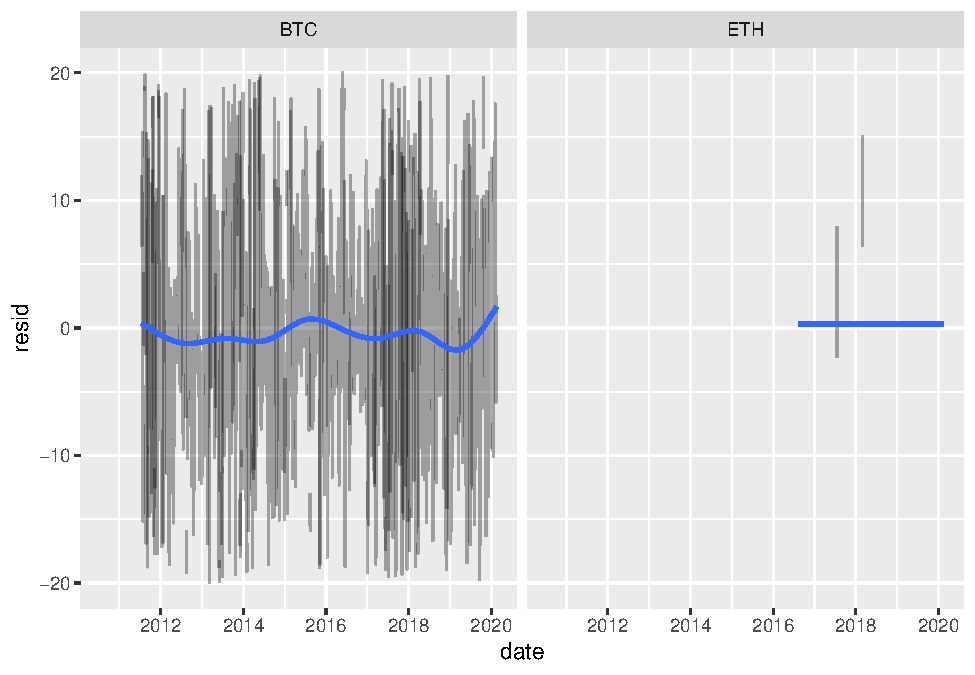
\includegraphics{RStudio-Internship-Application_files/figure-latex/unnamed-chunk-24-1.pdf}

\hypertarget{add-error-metrics-using-broom-r-broom}{%
\subsection{\texorpdfstring{Add error metrics using \texttt{broom} \citep{R-broom}:}{Add error metrics using broom {[}@R-broom{]}:}}\label{add-error-metrics-using-broom-r-broom}}

\begin{Shaded}
\begin{Highlighting}[]
\NormalTok{crypto_models_metrics <-}\StringTok{ }\NormalTok{crypto_data_grouped }\OperatorTok\StringTok{ }\KeywordTok{mutate}\NormalTok{(}\DataTypeTok{metrics=}\KeywordTok{map}\NormalTok{(model,broom}\OperatorTok{::}\NormalTok{glance)) }\OperatorTok\StringTok{ }\KeywordTok{unnest}\NormalTok{(metrics)}
\end{Highlighting}
\end{Shaded}

Sort by the best scores:

\begin{Shaded}
\begin{Highlighting}[]
\NormalTok{crypto_models_metrics }\OperatorTok\StringTok{ }\KeywordTok{arrange}\NormalTok{(}\OperatorTok{-}\NormalTok{r.squared)}
\end{Highlighting}
\end{Shaded}

\begin{verbatim}
## # A tibble: 2 x 15
## # Groups:   symbol [2]
##   symbol data  model resids r.squared adj.r.squared  sigma statistic  p.value
##   <chr>  <lis> <lis> <list>     <dbl>         <dbl>  <dbl>     <dbl>    <dbl>
## 1 BTC    <tib~ <lm>  <tibb~    0.158        0.148     12.4     16.1  4.47e-90
## 2 ETH    <tib~ <lm>  <tibb~    0.0341       0.00552 3203.       1.19 1.99e- 1
## # ... with 6 more variables: df <int>, logLik <dbl>, AIC <dbl>, BIC <dbl>,
## #   deviance <dbl>, df.residual <int>
\end{verbatim}

\hypertarget{how-much-better-do-the-models-get-if-we-add-more-variables}{%
\subsection{How much better do the models get if we add more variables?}\label{how-much-better-do-the-models-get-if-we-add-more-variables}}

Add MA, EMA, etc\ldots{}

\hypertarget{next-steps}{%
\subsection{Next Steps:}\label{next-steps}}

I won't go further than this here, but as my next steps, here is what I would do:

\begin{enumerate}
\def\labelenumi{\arabic{enumi}.}
\item
  Use parsnip + purrr to iterate through lots of predictive models
\item
  How much better do the models get with hyperparameter tuning?
\item
  Visualize the best model before and after parameter tuning and then do the same with the worst performing model
\end{enumerate}

\hypertarget{build-interactive-learnr-tutorials-for-python-using-reticulate}{%
\section{Build interactive learnr tutorials for Python using reticulate}\label{build-interactive-learnr-tutorials-for-python-using-reticulate}}

I think I could be a great fit for the third project listed related to creating learnr tutorials for Python using reticulate. I have a fair amount of experience in Python, but it's never really clicked very much for as much as R in the past, and I am looking to step-up my Python skills. My Master's in Data Science will work with Python a lot, and people immediately ask if I make tutorials in Python when I show them the R tutorials I have made, so this would be a great one for me to work on. I am also constantly told that Python is better than R for the incorrect reasons, and being more of an expert in Python would certainly help me debunk that myth when someone makes that argument.

I am very familiar with the \texttt{reticulate} package and I have used it in the past in an RMarkdown file to make automated cryptocurrency trades through a Python package \texttt{shrimpy-python}, which worked really well: \url{https://github.com/shrimpy-dev/shrimpy-python}

Since I have already demonstrated my familiarity with learnr tutorials \textbf{\protect\hyperlink{learnr}{in the previous section}}, I will keep going with the code from the tidymodels project example I just finished and use Python for \ldots{} ADD GOAL HERE \ldots{}

DEV:

Replace this with the Python one:

Could make a very simple xgboost model maybe?

Could also show using Shrimpy API to pull latest data, manipulate in pandas and visualize

Mention experience/courses taken in Python and how it's never clicked with me very much but how I am taking a basic Python course in my Master's in Data Science and I am looking to take it as an opportunity to create a lot of content using reticulate.

\begin{Shaded}
\begin{Highlighting}[]
\KeywordTok{library}\NormalTok{(reticulate)}
\end{Highlighting}
\end{Shaded}

\hypertarget{about-me}{%
\chapter{About Me}\label{about-me}}

My formal education is more oriented towards business, but during my time in college I tried to focus on learning tangible skills as much as possible, and computer science/programming started becoming more my niche over time vs.~business. I am working towards a Master's in Data Science at the University of Denver and I live in Boulder, Colorado.

I was born and raised in Milan, Italy and moved to the middle of Manhattan with my American mom when I was 16 where I finished highschool. I ended up coming to Boulder after reading a \href{http://www.scottjurek.com/eat-run}{book about ultra marathon running} and I could really see myself living in Boulder running with a husky dog training for ultra marathons, so that's what I did:

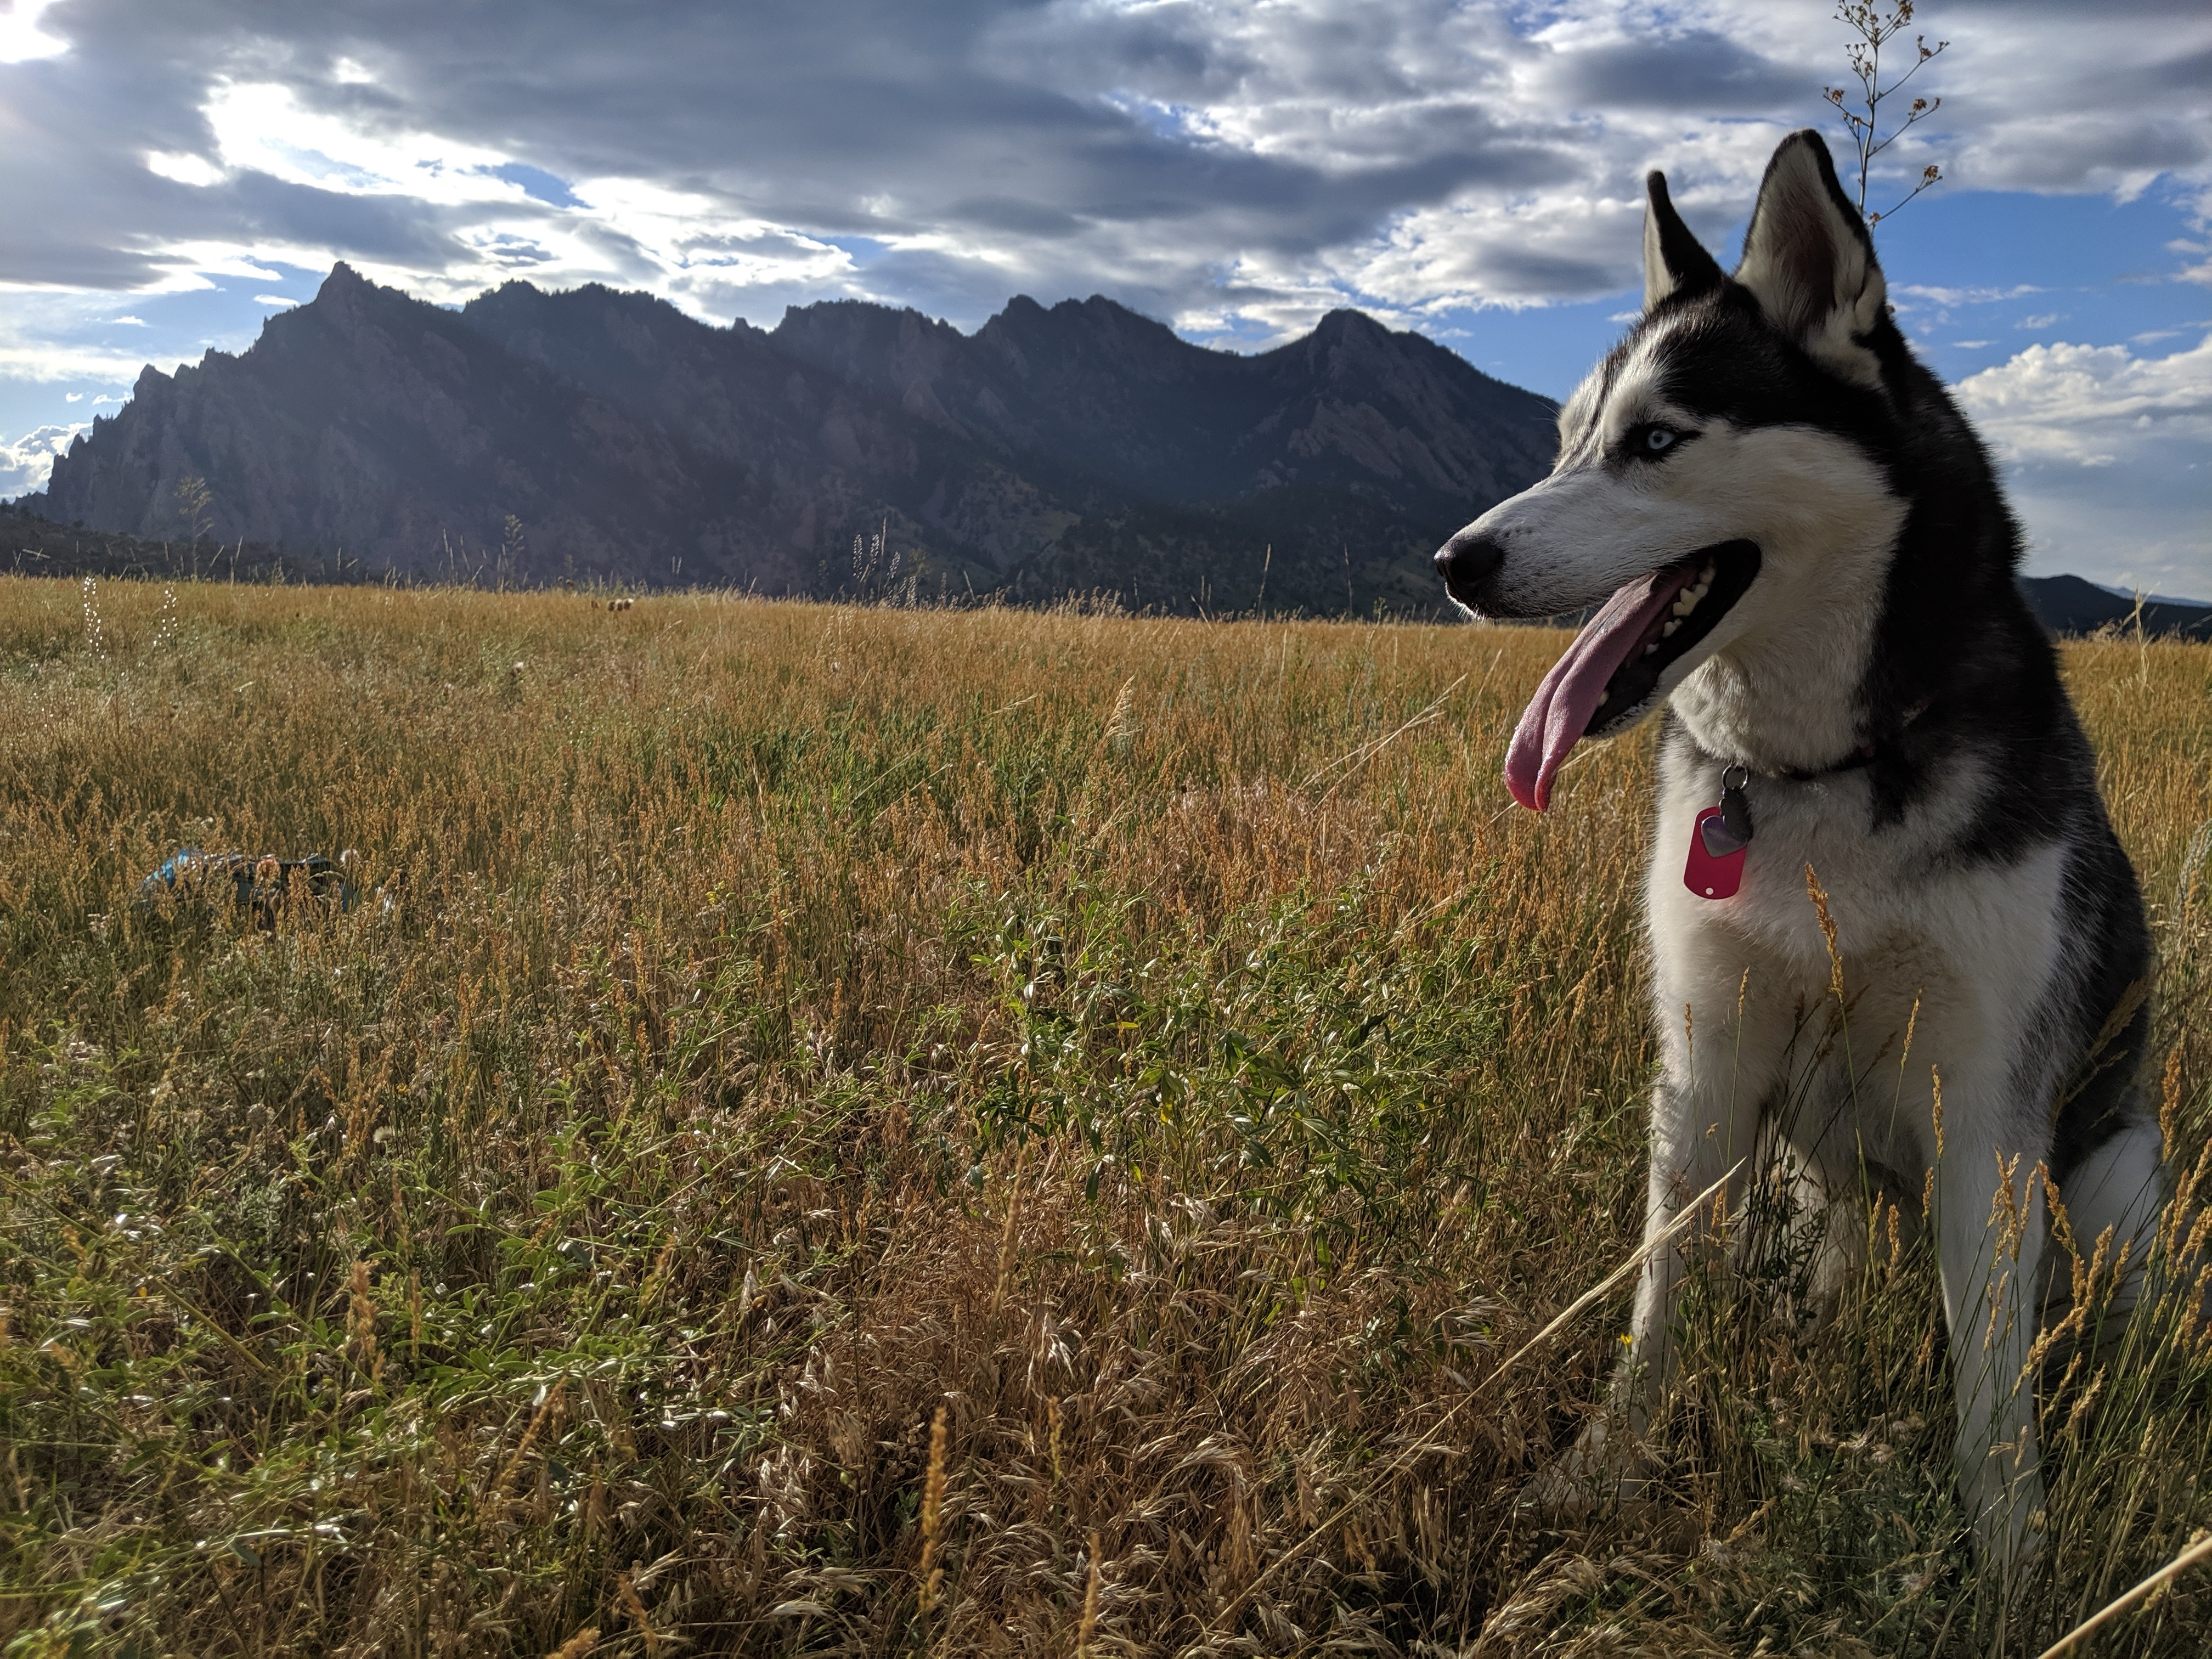
\includegraphics{images/sakura_option1.jpg}

I also have an adorable little ferret called Percy:

Is Sakura picture option 2 better?
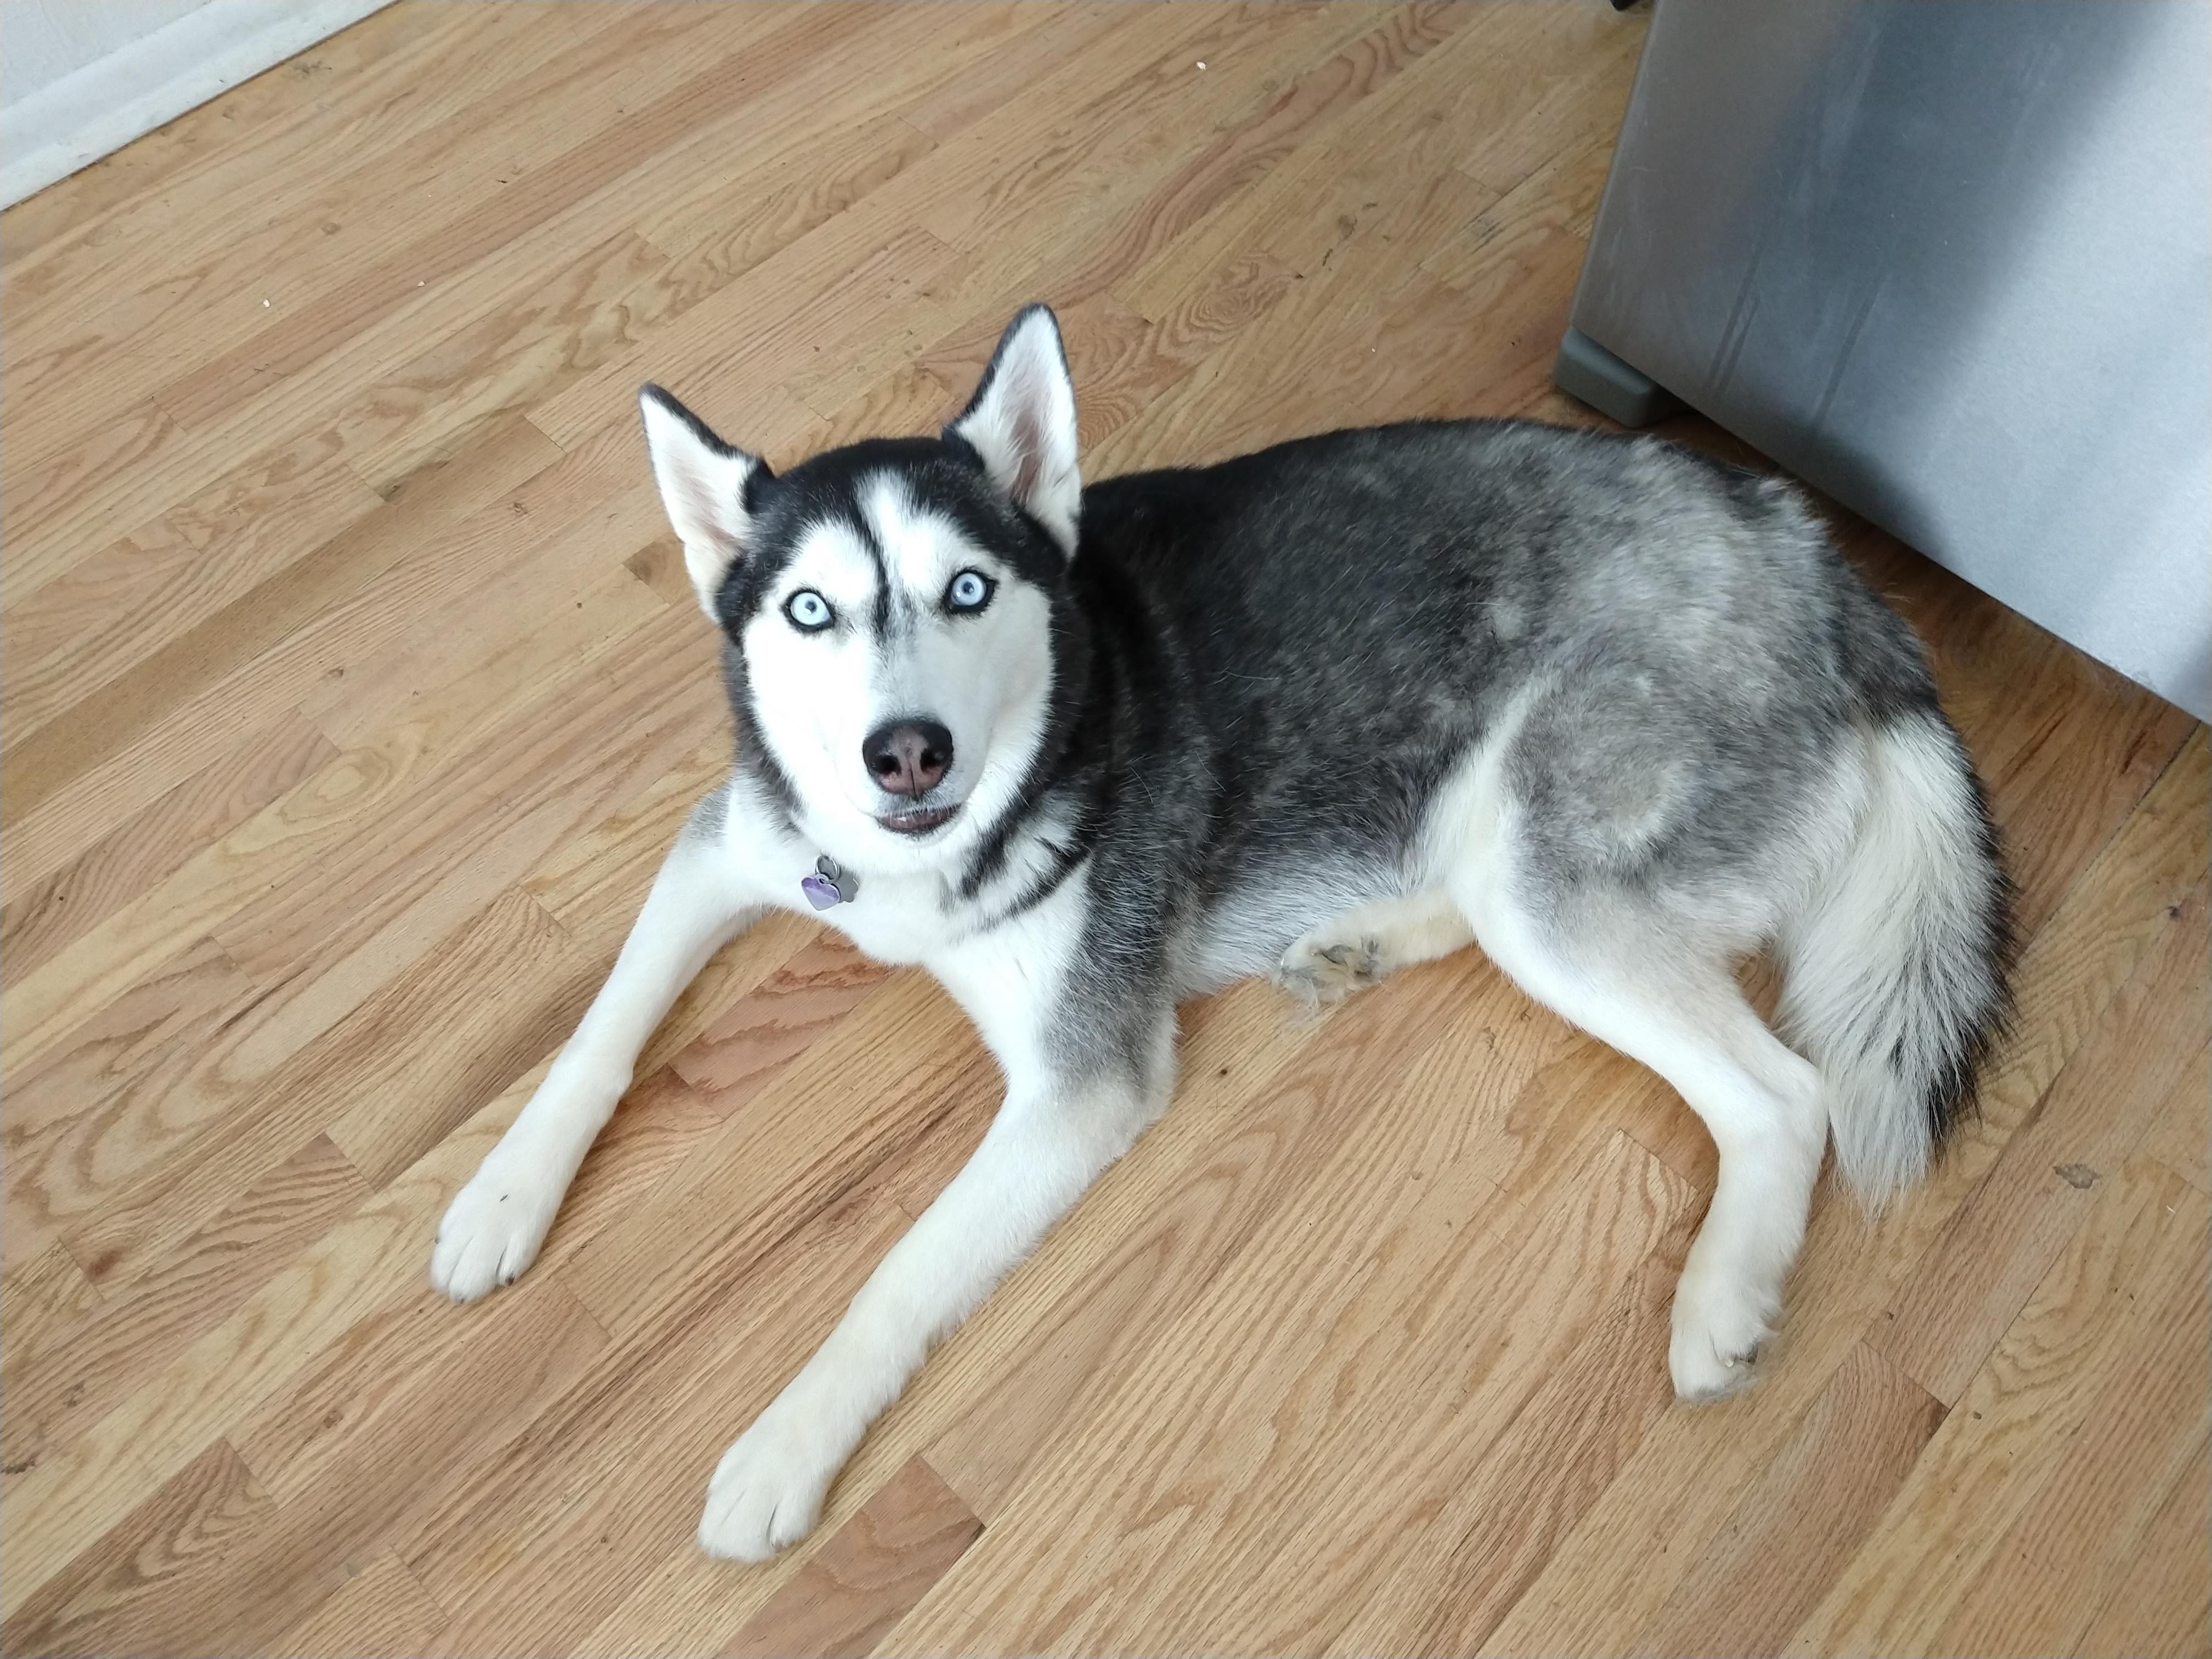
\includegraphics{images/sakura_option2.jpg}

I spent my time as an undergrad at the University of Colorado, Boulder studying information management and being a part of the \href{https://www.cutriathlon.com/}{CU Triathlon club team}. As a Junior at CU I was one of the TA's for MGMT 3200 (Business Analytics) after \textbf{\emph{really}} enjoying the course, which used Alteryx for doing ETL work, and a tool called \href{https://www.datarobot.com/}{DataRobot} for making predictions. The grade obtained by students in the class was strongly impacted by their team's percentile ranking on the leaderboards of real \href{https://www.kaggle.com/}{Kaggle} competitions that were going on at the time, and I found myself really loving working with data and I have been trying to learn as much as I can about anything and everything relating to data science since then. I spent multiple summers locking myself 40+ hours a week in my office working on just that.

Here are some of the online courses I worked my way through:

\begin{itemize}
\item
  \url{https://resclapon.com/datacamp-certificates}
\item
  \url{https://resclapon.com/udemy-certificates}
\end{itemize}

Here is my resume with the same online learning certificates added:

\begin{Shaded}
\begin{Highlighting}[]
\NormalTok{knitr}\OperatorTok{::}\KeywordTok{include_url}\NormalTok{(}\StringTok{"https://ricky-cv.netlify.com/"}\NormalTok{)}
\end{Highlighting}
\end{Shaded}

\href{https://ricky-cv.netlify.com/}{
\includegraphics{RStudio-Internship-Application_files/figure-latex/unnamed-chunk-27-1.pdf}}

In my senior year at CU Boulder, I did a business analytics internship with the Pricing Analytics team at Vail Resorts, which turned out to be a lot of manual work that should have been automated, so that's what I did. After graduating from CU Boulder I spent some time applying the things I learned around automation and web scraping to setup a project to collect data relating to the cryptocurrency markets from several sources because I had been trading on them since early 2014 and I saw an opportunity for some automated trading, and I wanted to have a personal project that I could work on over a longer period of time and use to get more comfortable in tools like SQL, R and Python with the prospect of making some money in the end. After a year and a half of working on this, I realized that I was actually better off opening up my project to others more and using it as a tool to teach others to program and that could be really valuable in my career progression towards eventually being a competent data scientist rather than spending all of my energy trying to make short-term trades, which doesn't really teach any tangible or useful skills outside of its own domain. The tutorials and lessons I am building specifically around this project can be found on \url{https://predictcrypto.org/}.

Today I am working towards a master's in Data Science part-time online and working on creating more research (including a more legitimate research paper with two professors) around the \emph{PredictCrypto} project, and working on putting out more \href{https://www.youtube.com/channel/UCZKbm8LERZBe_hwJNwroCPg?view_as=subscriber}{tutorials and content through a YouTube channel}. My master's program allows me to take one course at a time, be a full-time student, or do anything in between, so that flexibility allows me to work full-time without having an overwhelming schedule.

\hypertarget{ideal-tutorial}{%
\chapter{Ideal Tutorial}\label{ideal-tutorial}}

\hypertarget{overview-1}{%
\section{Overview}\label{overview-1}}

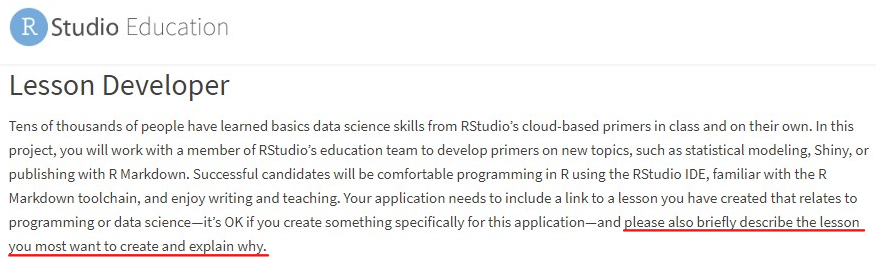
\includegraphics{images/idealTutorial.png}

I don't see this question on the last post regarding the RStudio internship applications being open through March 6th, but I have been thinking about this question since I saw it \href{https://education.rstudio.com/blog/2019/11/rstudio-internships-2020-preview/}{originally posted here in November}, so I wanted to include this answer in my application.

Ultimately I think analyzing cryptocurrencies is fun and interesting and a good way to get people's attention, but I have been thinking that a much more useful application of these ideas would be to be able to do a very similar thing but to create live data feeds from sensors out in the real world. This data could then be used to provide highly interactive programming tutorials, where the outcomes of the analysis would change based on the most recent data that was collected. To give a practical example of what that could look like, if there was a live data feed of sensors across Australia giving live information around particulates, carbon monoxide, ozone, carbon dioxide as well as other factors like informaton about the wind, etc.. it seems to me that this could empower things like early detection and much better prevention in general through predictive modeling and being able to triangulate the location of fires as they start or to figure out how to spread the limited resources across the different fires, and I just love the idea of the possibility of moving the needle on a problem through programming tutorials rather than working with uninteresting old data. Creating a system that allows people to actually contribute towards solving real problems might be wishful thinking, but I do believe that the best to teach someone these concepts is to give them data they care about and give them a realistic path forward to apply their existing intuition to answer questions they care about. The \texttt{mtcars} and \texttt{iris} datasets are great, but data feeds that change over time would be better in \textbf{\emph{some}} cases in terms of getting a person invested in the actual analysis being done.

\hypertarget{tutorials-planned}{%
\section{Tutorials I Have Planned}\label{tutorials-planned}}

As I was thinking through this question, I realized that beyond doing cool work around the data being used itself, I have a pretty lengthy list of topics that I feel are not always expressed as concisely as they should be. These topics \emph{have} been covered by others in the past, but if I had a 5-10 minute video outlining things the way I plan on doing it, it would have saved me a lot of time, so hopefully even if I only reach a couple of people I will have saved them a lot of time, as well as myself whenever I want to go back to using \textbf{any of these tools:}

\begin{itemize}
\item
  Creating a website with bookdown, GitHub and Netlify.

  \begin{itemize}
  \tightlist
  \item
    Conceptually speaking this is amazingly simple to implement if you just know where to click in GitHub + RStudio and does things that would be pretty difficult to achieve with older tools.
  \end{itemize}
\item
  GitHub actions for automation

  \begin{itemize}
  \item
    This is a pretty new topic because GitHub Actions have been very recently introduced and most resources online make this way overcomplicated and/or they are not usually specific to R. It's actually not that difficult though and it makes a ton of sense conceptually, especially when using \texttt{devtools::check()}, and is a general tool that can be used for all sorts of automation. In fact, it would be a terrible experience, but you could program in R without needing your own computer by using GitHub actions.
  \item
    I was running into an issue I did not understand when using GitHub actions with bookdown files because of the default argument \texttt{clean\_envir=FALSE} when running \texttt{render\_book()}, and I documented the issue here: \url{https://community.rstudio.com/t/github-actions-object-from-secrets-not-found/54519/5}
  \item
    After making a video tutorial around making a website with bookdown, I plan on using that project to explain github actions in another video.
  \end{itemize}
\item
  Using blogdown and pagedown
\item
  Making an R package
\item
  Creating tests to go along with an R package

  \begin{itemize}
  \tightlist
  \item
    Including code coverage and having the custom badge on the GitHub page refreshed through GitHub actions
  \end{itemize}
\item
  General overview of how to use GitHub with RStudio

  \begin{itemize}
  \tightlist
  \item
    In companies you would have a development space and a \textbf{production} environment and I see my personal use of GitHub + RStudio as being very similar to that. When you make changes locally it's conceptually similar to a dev environment, and when you push things to GitHub those changes are published to the production environment where it has downstream effects, for example triggering a new build for a website.
  \end{itemize}
\item
  Setting up R + RStudio + GitHub

  \begin{itemize}
  \item
    Downloading R
  \item
    Downloading RStudio
  \item
    Downloading GitHub and pointing the global options within RStudio to point to git.exe to prompt RStudio to ask for login and create the \textbf{Git} tab in the IDE
  \end{itemize}
\item
  Flexdashboards
\item
  Web Scraping
\item
  Using RStudio Add-Ins and coolest ones
\item
  Awesome ggplot2 extensions

  \begin{itemize}
  \item
    trelliscope
  \item
    rayshader + rayrender
  \item
    ggmap
  \item
    gganimate
  \item
    gghighlight
  \item
    \ldots{} LOTS more
  \end{itemize}
\item
  Understanding the tidyverse. Here's a quick example of the things I would really drive home in a tutorial around the tidyverse and when/why you would want to use the pipe operator:
\end{itemize}

Take the following example:

\begin{Shaded}
\begin{Highlighting}[]
\KeywordTok{sqrt}\NormalTok{(}\DecValTok{25}\NormalTok{)}
\end{Highlighting}
\end{Shaded}

\begin{verbatim}
## [1] 5
\end{verbatim}

Here it is easy enough to keep track of what is happening. We are taking the square root of 25 and nothing more. But let's say we have a more complex operation:

\begin{Shaded}
\begin{Highlighting}[]
\KeywordTok{abs}\NormalTok{(}\KeywordTok{exp}\NormalTok{(}\KeywordTok{sqrt}\NormalTok{(}\DecValTok{25}\NormalTok{)))}
\end{Highlighting}
\end{Shaded}

\begin{verbatim}
## [1] 148.4132
\end{verbatim}

As the code gets more complicated, it gets more difficult to read the code. What order do the operations run? Things can get pretty out of hand, this is not a particularly extreme example.

In comes the pipe operator! Using the \%\textgreater\% we \textbf{start} with the value being manipulated, and apply each operation one step at a time:

\begin{Shaded}
\begin{Highlighting}[]
\DecValTok{25} \OperatorTok\StringTok{ }
\StringTok{  }\KeywordTok{sqrt}\NormalTok{() }\OperatorTok\StringTok{ }
\StringTok{  }\KeywordTok{exp}\NormalTok{() }\OperatorTok\StringTok{ }
\StringTok{  }\KeywordTok{abs}\NormalTok{()}
\end{Highlighting}
\end{Shaded}

\begin{verbatim}
## [1] 148.4132
\end{verbatim}

Now it becomes much clearer that our code starts with the value 25 and the functions are applied in the order \texttt{sqrt()}, \texttt{exp()}, \texttt{abs()}.

When we work with a full dataset, this will also work much better because it will be much easier to distinguish between the data we want to apply a transformation to and the actual transformation. Let's walk through one more example to illustrate this idea.

Let's make a very simple example dataset:

\begin{Shaded}
\begin{Highlighting}[]
\NormalTok{data <-}\StringTok{ }\KeywordTok{data.frame}\NormalTok{(}\StringTok{"numbers"}\NormalTok{=}\KeywordTok{c}\NormalTok{(}\DecValTok{3}\NormalTok{,}\DecValTok{7}\NormalTok{,}\DecValTok{9}\NormalTok{))}
\NormalTok{data}
\end{Highlighting}
\end{Shaded}

\begin{verbatim}
##   numbers
## 1       3
## 2       7
## 3       9
\end{verbatim}

Without using the pipe operator, this is what the usage of the \texttt{filter()} function would look like:

\begin{Shaded}
\begin{Highlighting}[]
\KeywordTok{filter}\NormalTok{(data, numbers }\OperatorTok{>}\StringTok{ }\DecValTok{7}\NormalTok{)}
\end{Highlighting}
\end{Shaded}

\begin{verbatim}
##   numbers
## 1       9
\end{verbatim}

Treating the object \texttt{data} within the \texttt{filter()} function is not clear.
Using the pipe operator, this operation becomes more clear:

\begin{Shaded}
\begin{Highlighting}[]
\NormalTok{data }\OperatorTok\StringTok{ }\KeywordTok{filter}\NormalTok{(numbers }\OperatorTok{>}\StringTok{ }\DecValTok{7}\NormalTok{)}
\end{Highlighting}
\end{Shaded}

\begin{verbatim}
##   numbers
## 1       9
\end{verbatim}

To make this point clear, try to translate this code to english in your head:

\begin{Shaded}
\begin{Highlighting}[]
\KeywordTok{round}\NormalTok{(}\KeywordTok{log}\NormalTok{(}\KeywordTok{sqrt}\NormalTok{(}\KeywordTok{filter}\NormalTok{(data, numbers }\OperatorTok{>}\StringTok{ }\DecValTok{7}\NormalTok{))),}\DecValTok{3}\NormalTok{)}
\end{Highlighting}
\end{Shaded}

\begin{verbatim}
##   numbers
## 1   1.099
\end{verbatim}

Not exactly straightforward right? Now try to translate this code in your head and see if it is easier at all:

\begin{Shaded}
\begin{Highlighting}[]
\NormalTok{data }\OperatorTok
\StringTok{  }\KeywordTok{filter}\NormalTok{(numbers }\OperatorTok{>}\StringTok{ }\DecValTok{7}\NormalTok{) }\OperatorTok
\StringTok{  }\KeywordTok{sqrt}\NormalTok{() }\OperatorTok\StringTok{ }
\StringTok{  }\KeywordTok{log}\NormalTok{() }\OperatorTok\StringTok{ }
\StringTok{  }\KeywordTok{round}\NormalTok{(}\DecValTok{3}\NormalTok{)}
\end{Highlighting}
\end{Shaded}

\begin{verbatim}
##   numbers
## 1   1.099
\end{verbatim}

You could read this line by line as:

\begin{enumerate}
\def\labelenumi{\arabic{enumi}.}
\item
  Start with the dataframe object called \texttt{data}
\item
  Filter the rows based on the column called \texttt{numbers} having a value larger than 7
\item
  Take the square root of the result
\item
  Take the log of the result
\item
  Round the result by 3 decimal places
\end{enumerate}

\hypertarget{final-notes}{%
\section{Final notes}\label{final-notes}}

I would also have a version of \protect\hyperlink{tutorials-planned}{each planned tutorial} recorded in Italian, because I am bilingual and most of this content does not currently exist in Italian as far as I can tell.

\hypertarget{cool-charts}{%
\chapter{Cool Charts}\label{cool-charts}}

\hypertarget{disable-while-working-on-bookdown-takes-too-long-to-render}{%
\section{Disable while working on bookdown, takes too long to render!}\label{disable-while-working-on-bookdown-takes-too-long-to-render}}

Here are some examples of charts, which refresh daily using GitHub actions and Netlify for automation.

\begin{verbatim}
## [1] TRUE
\end{verbatim}

  \bibliography{book.bib,packages.bib,main.bib}

\end{document}
